\section{Definite integrals and Fundamental Theorem of Calculus}

In certain application scenarios, we would want to evaluate the area under the curve of a function (bounded by the $x$-axis).  For example, in economics, suppose we have supply and demand curves shown in the graph below, where $P$ stands for price, $Q$ stands for quantity, $D(Q)$ is the demand function, $S(Q)$ is the supply function, and $P^*$, $Q^*$ are the price and demand under equilibrium.  Then the \textit{consumer surplus} is defined as the shaded area marked with "CS", and the \textit{producer surplus} is defined as the shaded area marked with "PS".  It is then clear that the consumer surplus can be evaluated by subtracting $P^*Q^*$ from the area under $D(Q)$ from $Q = 0$ to $Q = Q^*$.  The producer surplus can be calculated as $P^*Q^*$ minus the area under $S(Q)$ from $Q = 0$ to $Q = Q^*$.  Therefore, it would be convenient if we could 
come up with a notation to express areas under curves and develop a technique to evaluate them.

\medskip
\begin{figure}[ht]
    \centering
    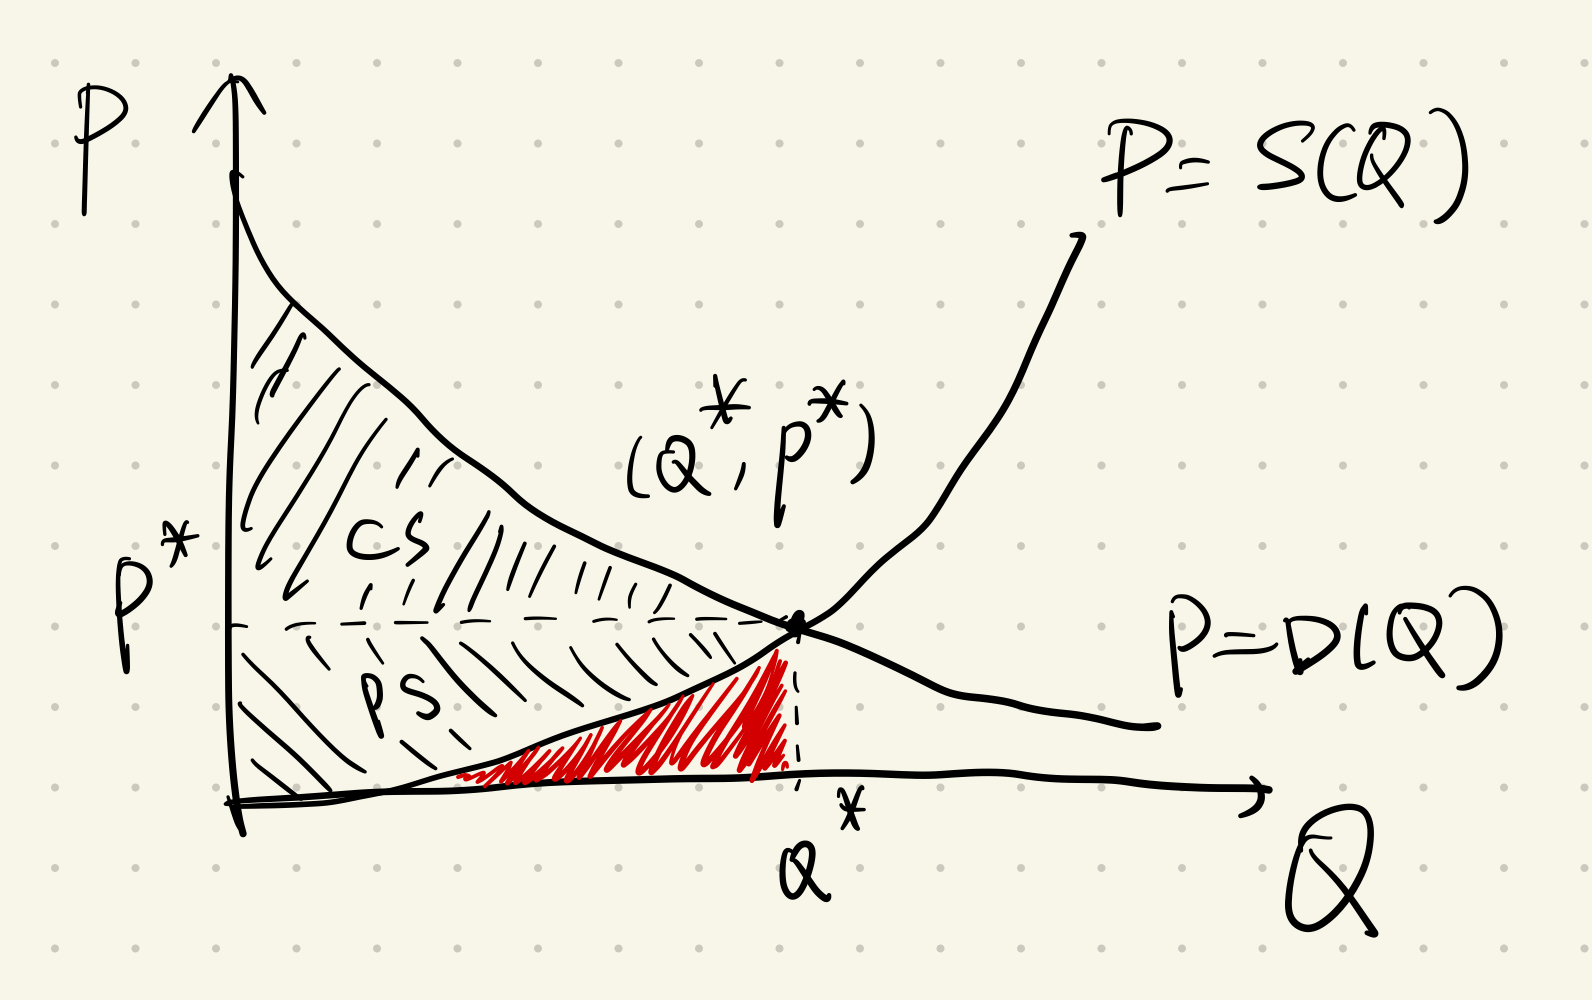
\includegraphics[width = 0.7\textwidth]{figures/chap 07/supply_demand.png}
\end{figure}

\medskip
A side note is that, in the example above, $D(Q)$ and $S(Q)$ are always positive, so it makes sense to talk about area \textit{under} the curve.  However, for functions taking negative values like the what the following graph depicts, the area bound by the curve and the $x$-axis is actually \textit{above} the curve.  In this case, for mathematical consistency, we use the notion of \textbf{signed area}, where areas above the curve and under the $x$-axis like this is given a negative sign.  With the concept of area-under-curve and signed area established, we can now define definite integrals as follows:

\begin{figure}[ht]
    \centering
    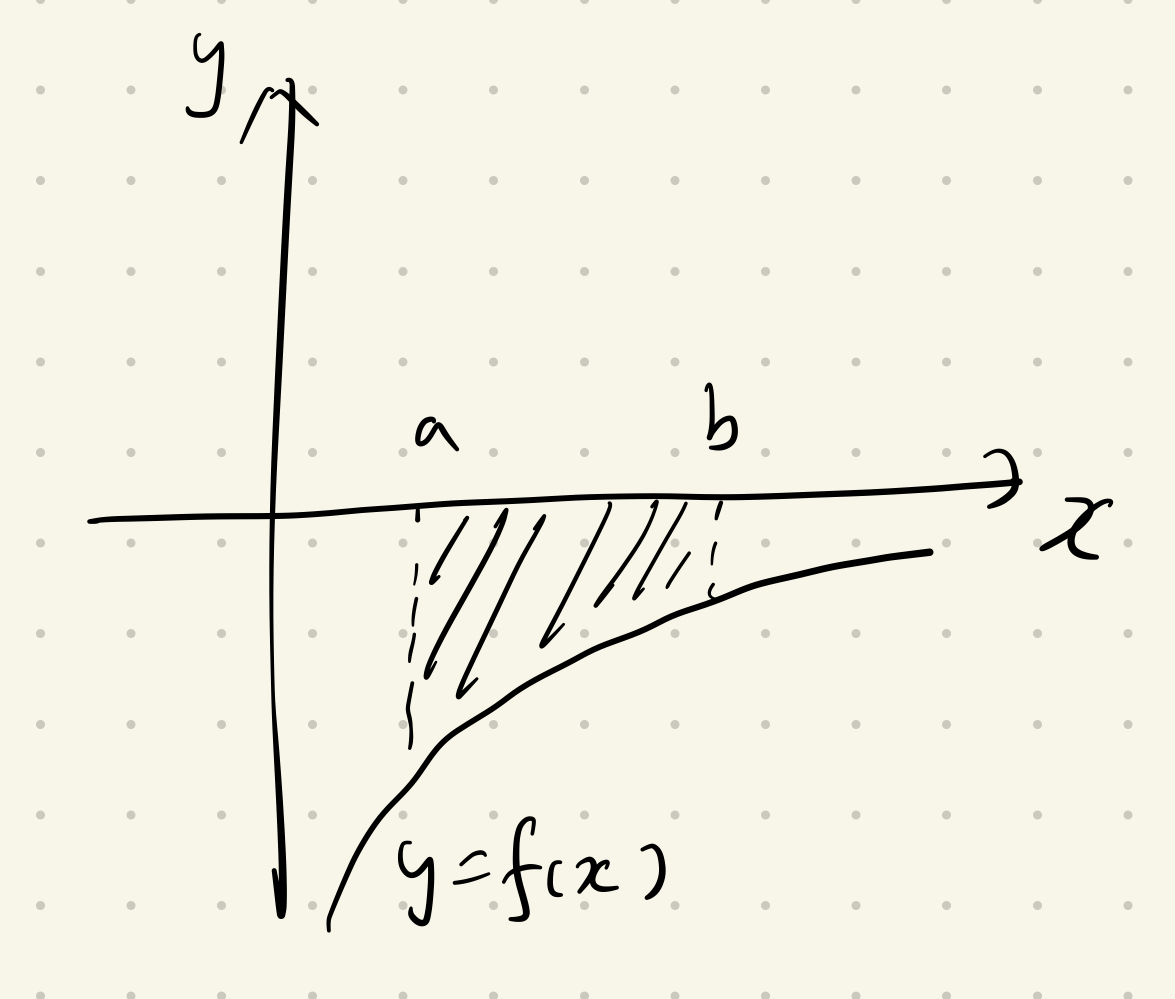
\includegraphics[width = 0.5\textwidth]{figures/chap 07/signed_area.png}
\end{figure}

\begin{defi}[Definite integrals]{def: definite_integral}
    Let $f(x)$ be a continuous function on a closed interval $[a,b]$.  The signed area bounded by the curve of $f(x)$, the $x$-axis, $x=a$ and $x=b$ is called the \textbf{definite integral} of $f(x)$ from $a$ to $b$, denoted by
    \[\int_a^b f(x)~dx\]
    where $a$ and $b$ are termed the lower and upper limit of integration for the definite integral.
\end{defi}

From this definition, if we go back to our previous example, we can notate the cosumer and producer surplus by:
\begin{align*}
    \text{Consumer surplus} &= \Big[\int_0^{Q^*} D(Q) dQ\Big] - P^*Q^*\\
    \text{Producer surplus} &= P^*Q^* - \Big[\int_0^{Q^*} S(Q) dQ\Big]
\end{align*}

Note that since definite integrals represent areas under curve, we have the following identities for definite integrals:
\begin{itemize}
    \item $\int_a^b kf(x)~dx = k\int_a^b f(x)~dx$
    \item $\int_a^b [f(x) \pm g(x)]~dx = \int_a^b f(x)~dx \pm \int_a^b g(x)~dx$
    \item $\int_a^b f(x)~dx = \int_a^c f(x)~dx + \int_c^b f(x)~dx$
    \item $\int_a^a f(x)~dx = 0$
    \item $\int_a^b f(x)~dx = -\int_b^a f(x)~dx$
\end{itemize}
where in the third identity, the area under $f(x)$ between $x = a$ and $x = b$ is intuitively decomposed into the sum of area under curve between $x = a$ and $x = c$, and area under curve between $x = c$ and $x = b$.  Setting $c = a$ in the third identity would lead to 
\[\int_a^b f(x)~dx = \int_a^a f(x)~dx + \int_a^b f(x)~dx\]
\[0 = \int_a^a f(x)~dx\]
which is exactly the fourth identity.  Setting $b = a$ in the third identity would instead lead to
\[\int_a^a f(x)~dx = \int_a^c f(x)~dx + \int_c^a f(x)~dx\]
\[\int_c^a f(x)~dx = -\int_a^c f(x)~dx \]
which implies the fifth identity: switching the upper and lower limit of a definite integral adds a negative sign to it. 

Some definite integrals can be evaluated using our knowledge in geometry.  Let's look at the following examples:

\begin{eg}[]{eg: definite_integrals}
    Using the definition of definite integrals, evaluate the following expressions:
    \begin{tasks}(3)
        \task $\int_0^2 (3x+1)~dx$
        \task $\int_2^4 (2x-5)~dx$
        \task $\int_3^1 \sqrt{4-(x-1)^2}~dx$
    \end{tasks}
\end{eg}

\begin{egsol}[]{egsol: definite_integrals}
    \begin{enumerate}[a)]
        \item If we graph $f(x) = 3x+1$ on the Cartesian plane, we see that the area under the curve from $x=0$ to $x=2$ forms a trapezoid shown in the graph below.  The two bases of the trapezoid are $f(0) = 1$ and $f(2) = 7$, and its height is $2$, so the area would be $\frac{(7+1)\cdot 2}{2} = 8$.  Therefore, the definite integral evaluates to $8$.

        \medskip
        \begin{center}
            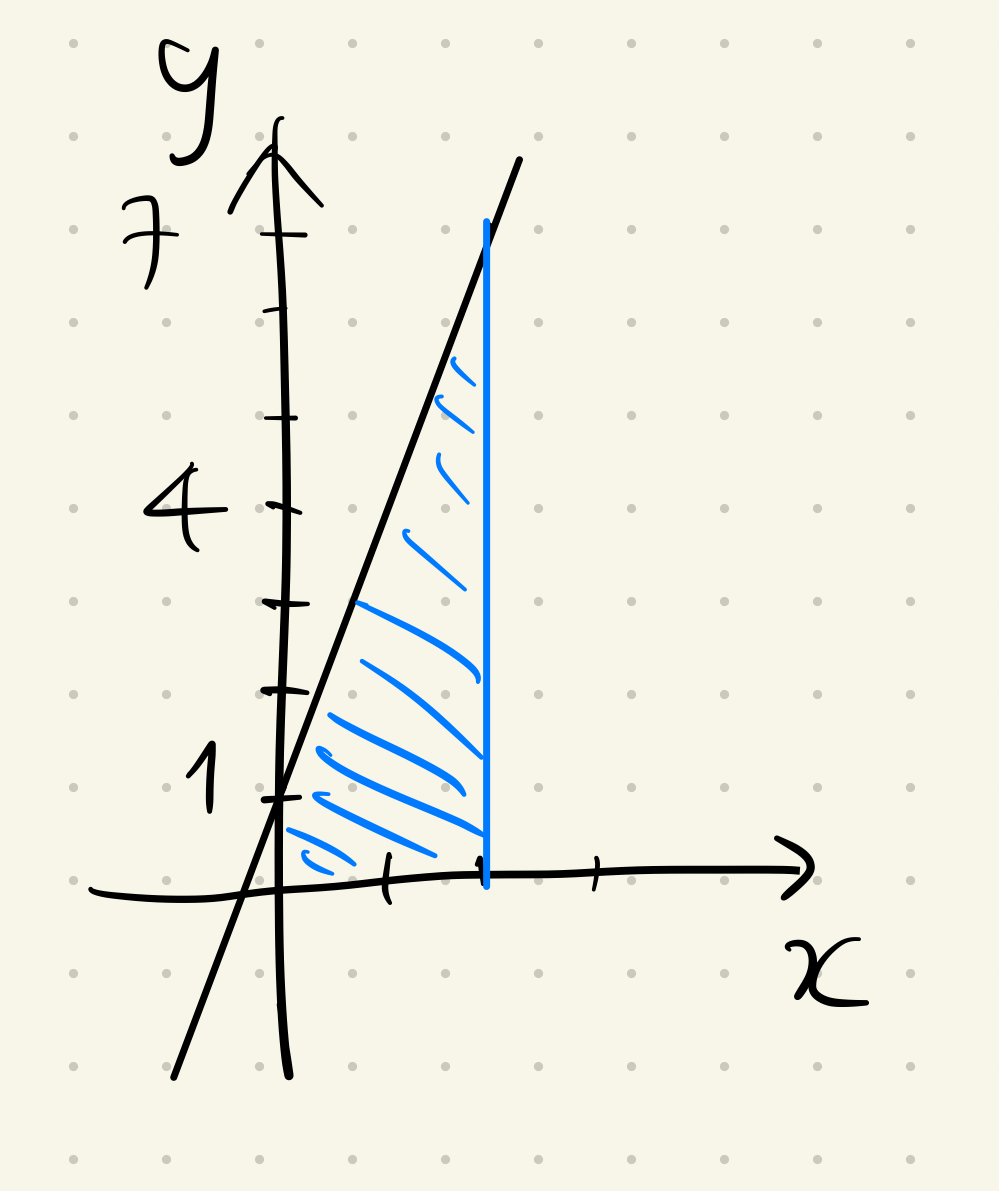
\includegraphics[width = 0.3\textwidth]{figures/chap 07/def_int_a.png}
        \end{center}
        \item If we graph $f(x) = 2x-5$ on the Cartesian plane, we see that between $x = 2$ and $x = 4$, part of the function is below the $x$-axis, and part of it is above the axis.  Since definite integrals are defined as signed area under the curves, we'll have to subtract the triangle below the axis from the triangle above the axis.  Using the identity of similar triangles, we know that since the height of the two triangles are $f(4) = 3$ and $|f(2)|=1$, their bases should be $2\cdot\frac{3}{1+3} = \frac{3}{2}$ and $2\cdot\frac{1}{1+3} = \frac{1}{2}$.  Therefore, the definite integral should evaluate to $\frac{3\cdot3/2}{2}-\frac{1\cdot1/2}{2} = 2$.
        
        \medskip
        \begin{center}
            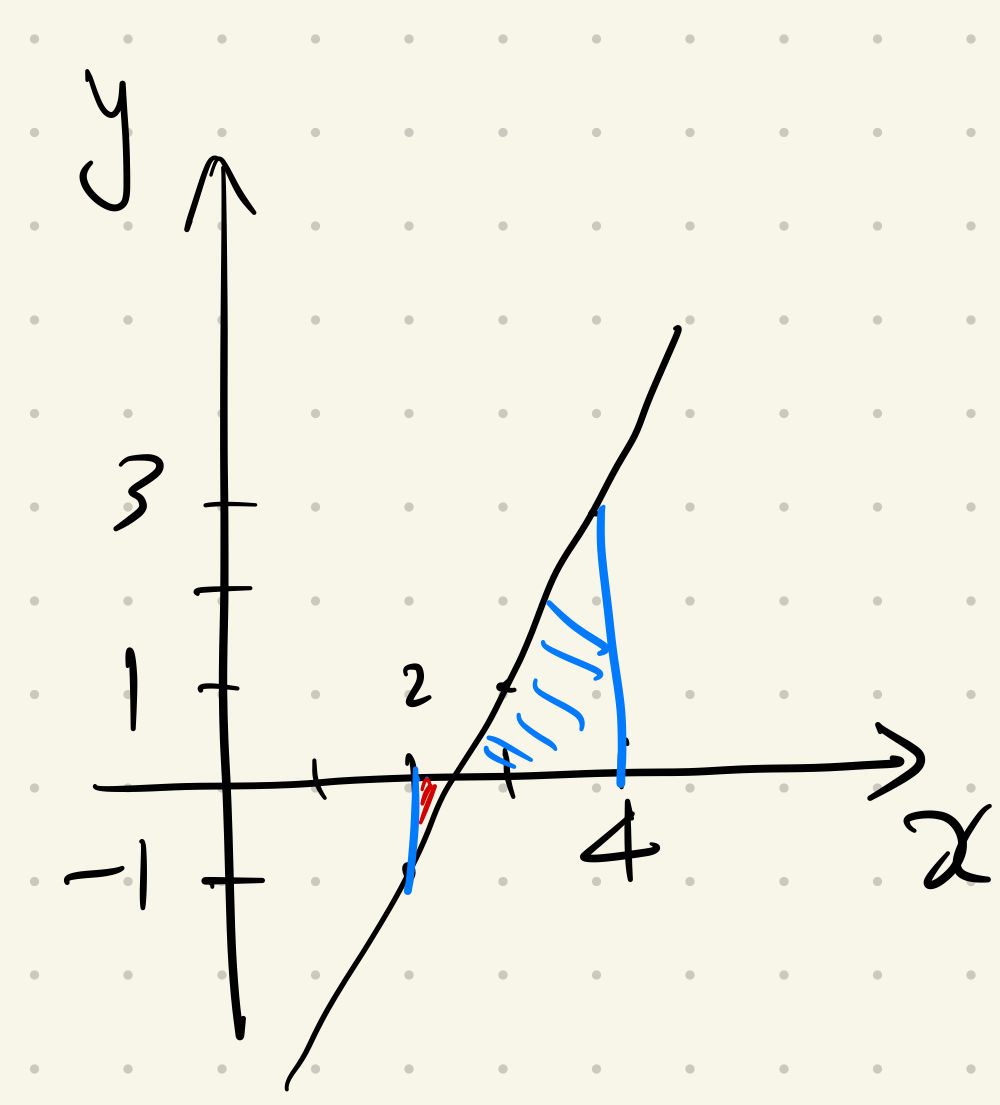
\includegraphics[width = 0.3\textwidth]{figures/chap 07/def_int_b.png}
        \end{center}
        \item Before we start graphing the function, note that upper limit of integration is smaller than its lower limit of integration, which is against our original definition.  However, using the identity we derived above, we can write
        \[\int_3^1 \sqrt{4-(x-1)^2}~dx = - \int_1^3 \sqrt{4-(x-1)^2}~dx\]
        Now the upper limit is larger than the lower limit, we can graph $f(x) = \sqrt{4 - (x-1)^2}$ on the Cartesian plane.  Rearranging $y = \sqrt{4 - (x-1)^2}$ yields $(x-1)^2 + y^2 = 2^2$, which implies that the curve of $f(x)$ is a half circle centered at $(1,0)$ with radius $2$.  Therefore, the area under the curve between $x=1$ and $x=3$ is a quarter of the circle, which has area $\pi\cdot(2)^2/4 = \pi$.  Therefore, our original definite integral evaluates to $-\pi$.
        
        \medskip
        \begin{center}
            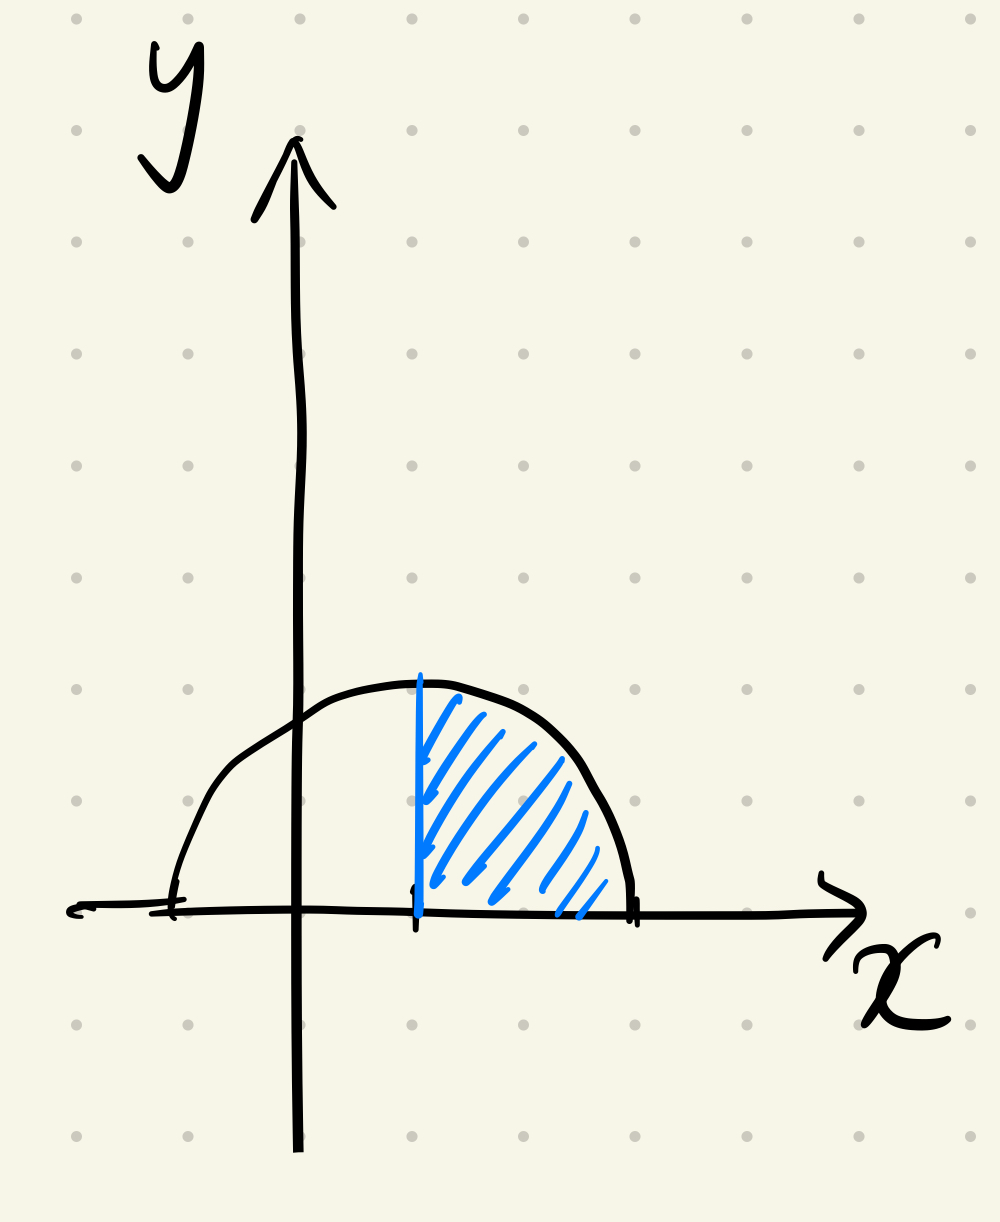
\includegraphics[width = 0.3\textwidth]{figures/chap 07/def_int_c.png}
        \end{center}
    \end{enumerate}
\end{egsol}

In the example above, the functions to be integrated represent straight lines and circles, so the area under the curves all formed shapes we are familiar with.  However, when the functions do not represent lines and circles, evaluating the integral will be much more difficult.  For example, suppose we would like to like to evaluate $\int_0^2 x^2~dx$, whose integrand is a upward-facing parabola as shown in the graph below.  One way to approach the area under curve is to first split the integration interval into smaller subintervals.  For example, in the graph, we split $[0, 2]$ into $8$ subintervals of length $\Delta x_{(8)} = 2/8$.  Then, the area under the curve can be approximated by the sum of the area of the blue bars, each with width $\Delta x_{(8)}$ and height $f(0 + j \Delta x_{(8)})$, where $j$ is the index of the subintervals ranging from $1$ to $8$.  We can write the approximation as
\begin{align*}
    \hat{A}_8 &= (f(0 + \Delta x_{(8)}) + f(0 + 2\Delta x_{(8)}) + f(0 + 3\Delta x) + ... + f(0 + 8 \Delta x_{(8)}))\Delta x_{(8)}\\
    &= \Big[\sum_{j=1}^8 f(0+j \Delta x_{(8)})\Big]\Delta x_{(8)}\\
    &= \Big[\sum_{j=1}^8 j^2 \Delta x_{(8)}^2\Big]\Delta x_{(8)}\\
    &= \Big[\sum_{j=1}^8 j^2\Big] \Delta x_{(8)}^3 =  \Big[\sum_{j=1}^8 j^2\Big] \Big(\frac{2}{8}\Big)^3 = 204 \cdot \Big(\frac{1}{4}\Big)^3 = \frac{51}{16}
\end{align*}

\begin{figure}[ht]
    \centering
    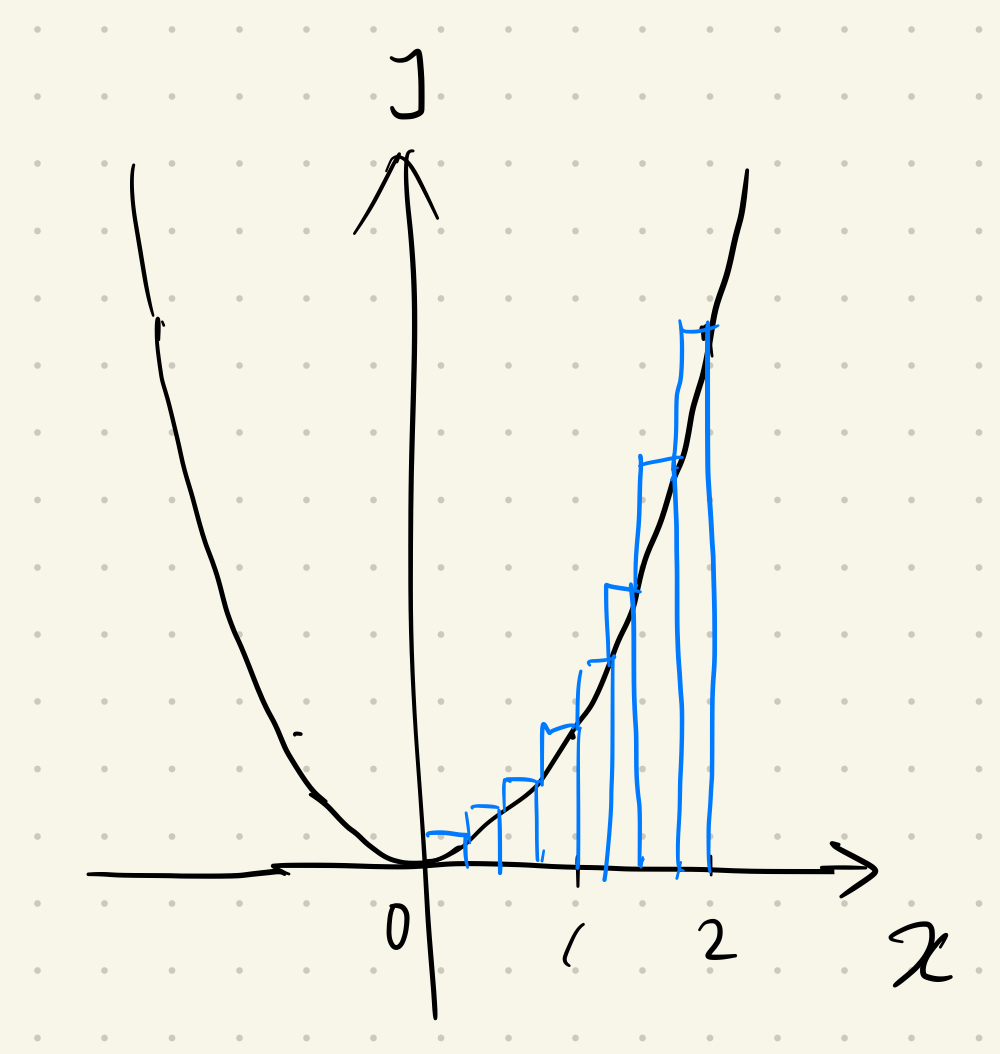
\includegraphics[width = 0.45\textwidth]{figures/chap 07/def_int_series.png}
\end{figure}

This approximation is called a (right) Riemann sum.  If we notate the number of subintervals as $n$ so that the length of the subintervals is $\Delta x_{(n)} = 2/n$, we yield a generalized Riemann sum:
\[\hat{A}_n = \Big[\sum_{j=1}^n j^2\Big] \Delta x_{(n)}^3 = \frac{n(n+1)(2n+1)}{6} \Big(\frac{2}{n}\Big)^3 = \frac{4n(n+1)(2n+1)}{3n^3}\]
where the second equality uses the formula for sum of squares of the first $n$ positive numbers.  Note as $n$ increases, the bars will be finer and finer, and the sum of the bars will eventually approach to the area under the curve.  Therefore, we can write our definite integral as a limit with $n$ approaching infinity:
\[\int_0^2 x^2~dx = \lim_{n \rightarrow \infty} \hat{A}_n = \lim_{n \rightarrow \infty} \frac{4n(n+1)(2n+1)}{3n^3} = \frac{8}{3}\]
where the last equality comes from the ratio of leading coefficients.

Here, we used the limit of Riemann sums to evaluate the definite integral, which is not an easy feat.  However, our success is not without luck: because our integrand is $x^2$, the sum of squares of the first $n$ positive numbers appeared in the Riemann sum, which we happened to know a clean formula for the sum.  If our integrand was something gnarlier, then it may well be the case that we do not have a closed form expression for the Riemann sum, and thus cannot take its limit.  In light of this, we will need a more general procedure to evaluate definite integrals. 

To develop the procedure, first we define an \textbf{area function} as a definite integral that leaves its upper limit as input.  For example, in the graph below, we define the area function $F(x) = \int_0^x f(t)~dt$, where the lower limit of integration is fixed at $0$ but the upper limit of integration is the variable $x$.  The signed area $F(x)$ represents is then by definition the area shaded blue.  

\begin{figure}[ht]
    \centering
    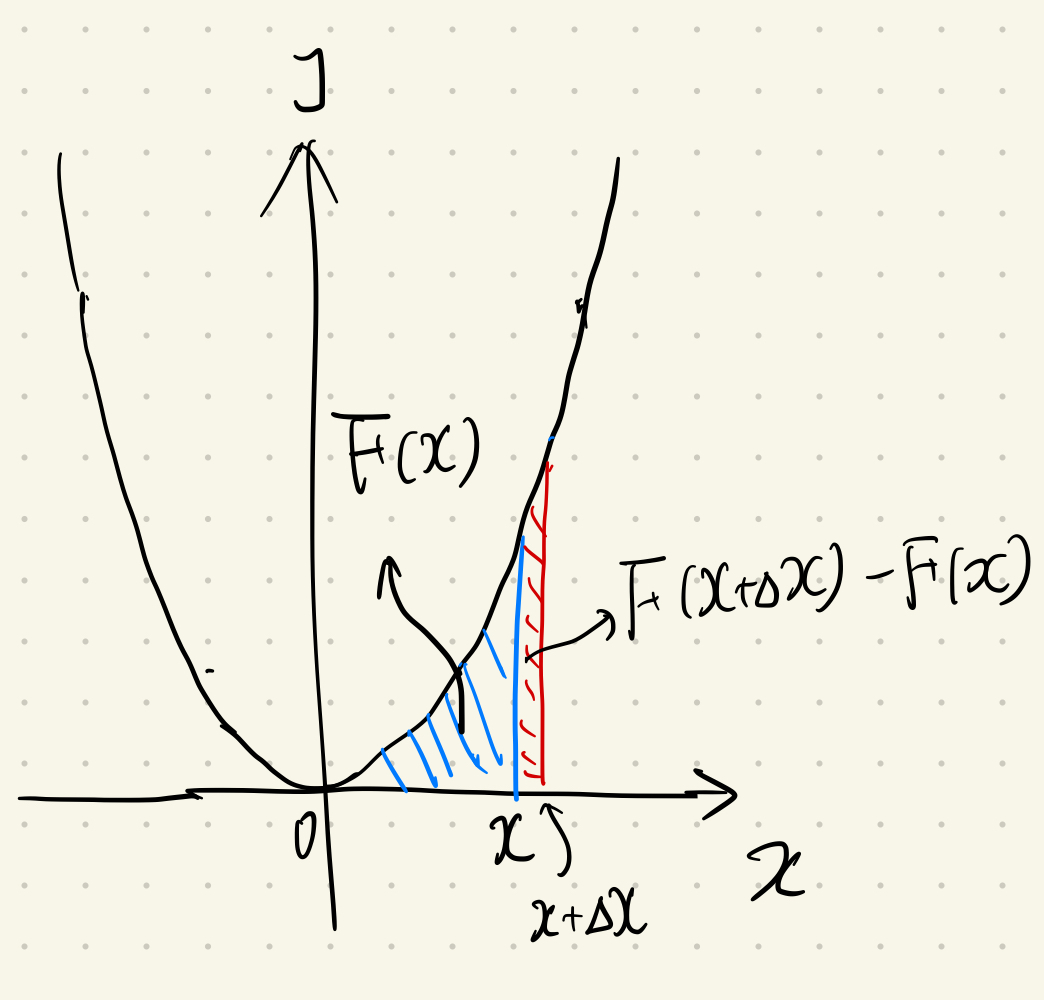
\includegraphics[width = 0.45\textwidth]{figures/chap 07/FTC.png}
\end{figure}

Now for a small $\Delta x$, the difference between $F(x+\Delta x)$ and F(x) would be the small strip of area under curve from $x$ to $x + \Delta x$, which is the area shaded red in the graph.  As $\Delta x$ gets smaller and smaller, the area of the strip would be closer and closer to $f(x) \Delta x$.  In other words, as $\Delta x$ gets smaller and smaller, the ratio between $F(x + \Delta x) - F(x)$ and $\Delta x$ would approach $f(x)$.  Therefore, we have

\[\frac{dF}{dx} = \lim_{\Delta x \rightarrow 0} \frac{F(x + \Delta x) - F(x)}{\Delta x} = f(x)\]

which implies that $F(x)$, which we originally defined as an area function, is actually an antiderivative of $f(x)$!  This remarkable result serves as a bridge between integral calculus (definite integrals) to differential calculus (antiderivatives), which we formally state in the theorem below:

\begin{theo}[Fundamental Theorem of Calculus, First Part]{thm: FTC1}
    Let $f(x)$ be a continuous function on $[a, b]$. Suppose $F(x)$ is an area function defined as 
    \[F(x) = \int_a^x f(t) dt, \quad x \in (a,b)\]
    then $F'(x) = f(x)$ for all $x \in (a,b)$.
\end{theo}

However, note that the first part of the Fundamental Theorem of Calculus only tells us that the area function $F(x)$ is \textit{an} antiderivative of $f(x)$, but does not tell us \textit{which} antiderivative it is.  That is, it does not explicitly tell us what the integration constant should be when we have obtained our antiderivative.  Fortunately, the second part of the Fundamental Theorem of Calculus tells us that as long as we are only interested in evaluating the definite integral, the choice of integration constant does not matter (it also relaxes the requirement for $f(x)$ to be continuous, but here we will not dig deeper into this issue):

\medskip
\begin{theo}[Fundamental Theorem of Calculus, Second Part]{thm: FTC2}
    Let $f(x)$ be a function on $[a, b]$.  Let $F(x)$ be \textit{any} antiderivative for $f(x)$, then
    \[\int_a^b f(x) dx = F(b) - F(a)\]
\end{theo}

Therefore, to find the definite integral for $f(x)$ from $a$ to $b$, we just need to find \textit{one} antiderivative for $f(x)$, and subtract its value at $x = b$ by its value at $x = a$.  Here since antiderivatives are closely linked to the evaluation of definite integrals, they are alternatively termed as \textbf{indefinite integrals}.

Let us try out our new evaluation method for definite integrals with a few examples:

\begin{eg}[]{eg: def_int_FTC}
    Evaluate the following definite integrals
    \begin{tasks}(3)
        \task $\int_0^2 x^2~dx$
        \task $\int_{\pi/2}^{0} \sin x~dx$
        \task $\int_1^{\sqrt{3}} \frac{1}{x^2+1}~dx$
        \task $\int_0^1 \frac{x}{x^2+1}~dx$
        \task $\int_{1/2}^{\sqrt{3}/2} \frac{1}{(\sqrt{1-x^2})^3}~dx$
        \task $\int_{0}^{\pi/4} x \cos x~dx$
    \end{tasks}
\end{eg}

\begin{egsol}[]{egsol: def_int_FTC}
    \begin{enumerate}[a)]
        \item We have evaluated this definite integral the hard way using Riemann sums.  Now let us try using antiderivatives and the Fundamental Theorem of Calculus.  Since one antiderivative of $x^2$ is $\frac{1}{3}x^3$, we can write:
        \[\int_0^2 x^2~dx = \frac{1}{3}x^3\Big]^2_0 = \frac{1}{3}(2)^3 - \frac{1}{3}(0)^3 = \frac{8}{3}\]
        where the notation $g(x)\big]^b_a$ stands for $g(b)-g(a)$.  Antiderivatives have indeed saved us much time here.
        \item Since one antiderivative of $\sin x$ is $-\cos x$, we have
        \[\int_{\pi/2}^0 \sin x~dx = (-\cos x)\Big]_{\pi/2}^0 = -\cos(0) + \cos(\pi/2) = -1 + 0 = -1\]
        Note here we do not even care if the upper limit of integration is larger than the lower limit.  We can just evaluate our antiderivatives with the correct order of subtraction, and the Fundamental Theorem of Calculus will take care of the rest.
        \item Remember that one antiderivative of $\frac{1}{x^2+1}$ is $\arctan x$, so we have
        \[\int_1^{\sqrt{3}} \frac{1}{x^2+1}~dx = \arctan x\Big]_1^{\sqrt{3}} = \arctan(\sqrt{3}) - \arctan(1) = \frac{\pi}{3} - \frac{\pi}{4} = \frac{\pi}{12}\]
        \item The antiderivative for this integrand is not immediately obvious, but if we try U-substituion with $u = x^2+1$, we have $du = 2xdx$, which works since the remainder of the integrand is $x$.  Therefore, we have
        \[\int_0^1 \frac{x}{x^2+1} dx = \frac{1}{2}\int_0^1 \frac{1}{x^2+1}(2xdx)\]
        Now note that when we preform variable substitutions in definite integrals, we will also have to substitute the limits of integration.  That is, originally we are integrating from $x = 0$ to $x = 1$, but now we are changing our variable for integration to $u$, the limits of integration should then be from $u = 0^2+1 = 1$ to $u = 1^2 + 1 = 2$.  We then yield
        \[\frac{1}{2}\int_0^1 \frac{1}{x^2+1}(2xdx) = \frac{1}{2} \int_1^2 \frac{1}{u} du = \frac{1}{2}(\ln |u|)\Big]_1^2 = \frac{1}{2}(\ln |2| - \ln |1|) = \frac{\ln 2}{2}\]
        \item The $\sqrt{1-x^2}$ in the denominator screams for a trigonometric substitution where $x = \sin \theta$ and $dx = \cos \theta d\theta$, but note that since we are performing variable substitution, we need to also transform the limits of integration.  This is where the range setting for $\theta$ becomes important.  Since we by convention set $-\pi/2 \le \theta \le \pi/2$, we have when $x = 1/2$ and $\sqrt{3}/2$, $\theta = \pi/6$ and $\pi/3$. Therefore we yield
        \begin{align*}
            \int_{1/2}^{\sqrt{3}/2} \frac{1}{(\sqrt{1-x^2})^3}~dx &= \int_{\pi/6}^{\pi/3} \frac{1}{\cos^3 \theta}\cos \theta d\theta\\
            &= \int_{\pi/6}^{\pi/3} \sec^2 \theta d\theta\\
            &= \tan \theta \Big]_{\pi/6}^{\pi/3}\\
            &= \tan\Big(\frac{\pi}{3}\Big) - \tan\Big(\frac{\pi}{3}\Big) = \sqrt{3} - \frac{1}{\sqrt{3}} = \frac{2}{3}\sqrt{3}
        \end{align*}
        \item Here the antiderivative can be found using integration by parts setting $u = x$ and $dv/dx = \cos x$, so that $du/dx = 1$ and $v = \sin x$.  Therefore we have
        \begin{align*}
            \int_{0}^{\pi/4} x \cos x~dx &= x \sin x \Big]_{0}^{\pi/4} - \int_{0}^{\pi/4} \sin x~dx\\
            &= x \sin x \Big]_{0}^{\pi/4} + \int_{0}^{\pi/4} (-\sin x)~dx\\
            &= x \sin x \Big]_{0}^{\pi/4} + \cos x \Big]_{0}^{\pi/4}\\
            &= \Big(\frac{\pi}{4} \sin \frac{\pi}{4} - 0 \sin 0\Big) + \Big(\cos \frac{\pi}{4} - \cos 0 \Big)\\
            &= \frac{\pi}{4} \cdot \frac{\sqrt{2}}{2} + \frac{\sqrt{2}}{2} - 1 = \frac{\sqrt{2}}{8}\pi + \frac{\sqrt{2}}{2}- 1
        \end{align*}
        Note that since this is a definite integral, the "$uv$" term is also subject to calculation of value difference at limits of integration, so don't forget to put a right bracket beside it!
    \end{enumerate}
\end{egsol}

\section{Area and arc length}

In the previous section we defined definite integrals as the area under the curve of a function, and showed that definite integrals can be promptly evaluated using antiderivatives.  However, definite integrals can do much more than calculating the area under the curve.  

To extend the use of definite integrals, first recall that back when we did not know how to use antiderivatives to evaluate definite integrals, we turned to the limit of Riemann sums, which can be written and graphed as follows 
\[\int_a^b f(x) dx = \lim_{\Delta x \rightarrow 0} \sum_{i=1}^n f(x_i) \Delta x\]
\begin{figure}[ht]
    \centering
    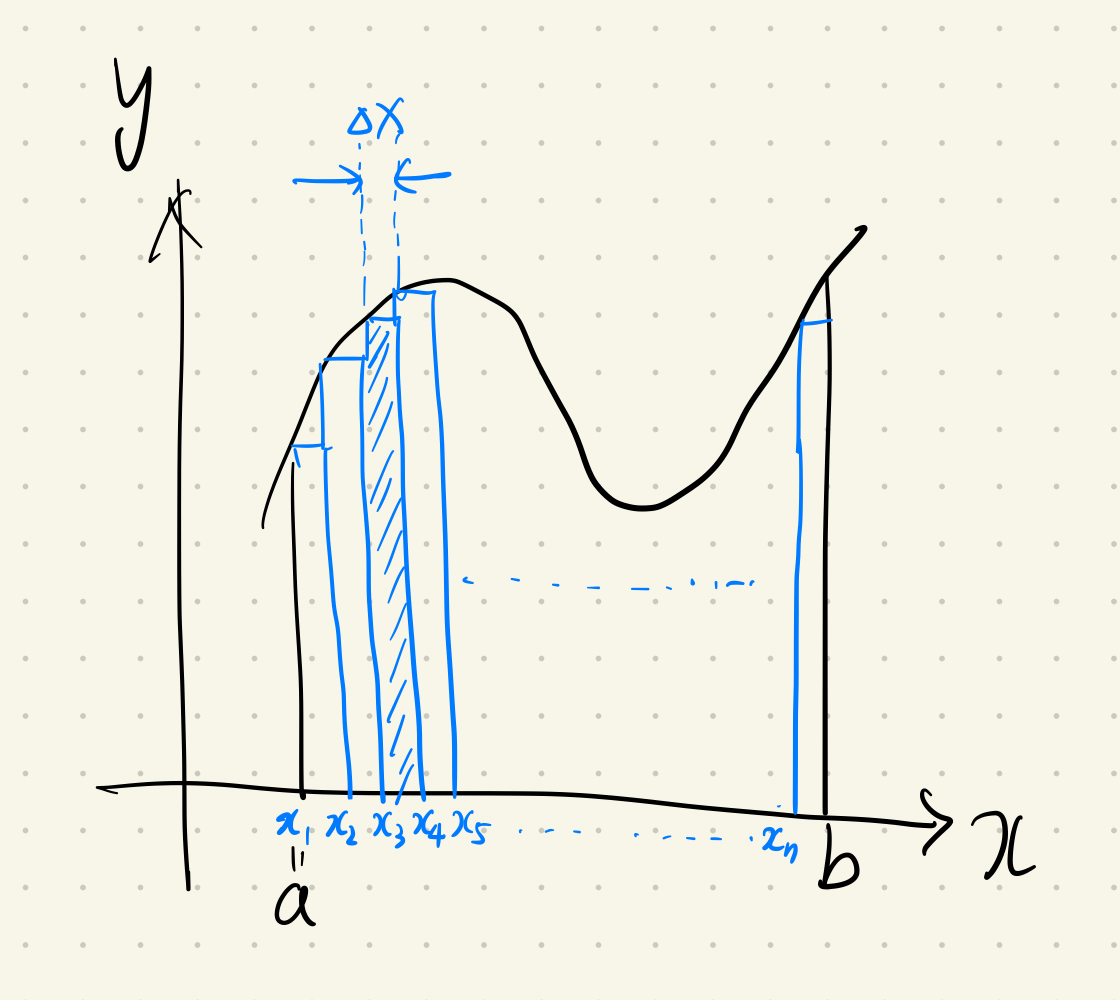
\includegraphics[width = 0.5\textwidth]{figures/chap 07/Riemann.png}
\end{figure}

\bigskip
In the right hand side, the term $f(x_i) \Delta x$ is the area of the strip of rectangle at $x = x_i$ with width $\Delta x$.  For example, $f(x_3)\Delta x$ represents the area of the blue strip shown in the graph.  Then, the summation sign adds all the strips up, with the $x$-coordinates of the strip ranging from $a$ to $b$.  Roughly speaking, as $\Delta x$ goes to zero, $f(x_i)\Delta x$ can be replaced with $f(x)dx$, and the summation sign can be replaced with $\int_a^b$, which re-frames the limit of summation into limit of integration.  The limit of integration specifies the limit of the variable indicated by the differential, which in this case is $x$.

With this correspondence in mind, we do not have to resort to writing out the limit of Riemann sums everytime we want to find a definite integral.  Instead, as shown in the left panel below, we can directly say that the area under $y = f(x)$ between $x = a$ and $x = b$ is just adding up the area of small shaded strips while $x$ goes from $a$ to $b$.  Since the area of the small strips is $f(x)dx$, we write the area as $\int_a^b f(x)dx$. 

\begin{figure}[ht]
    \centering
    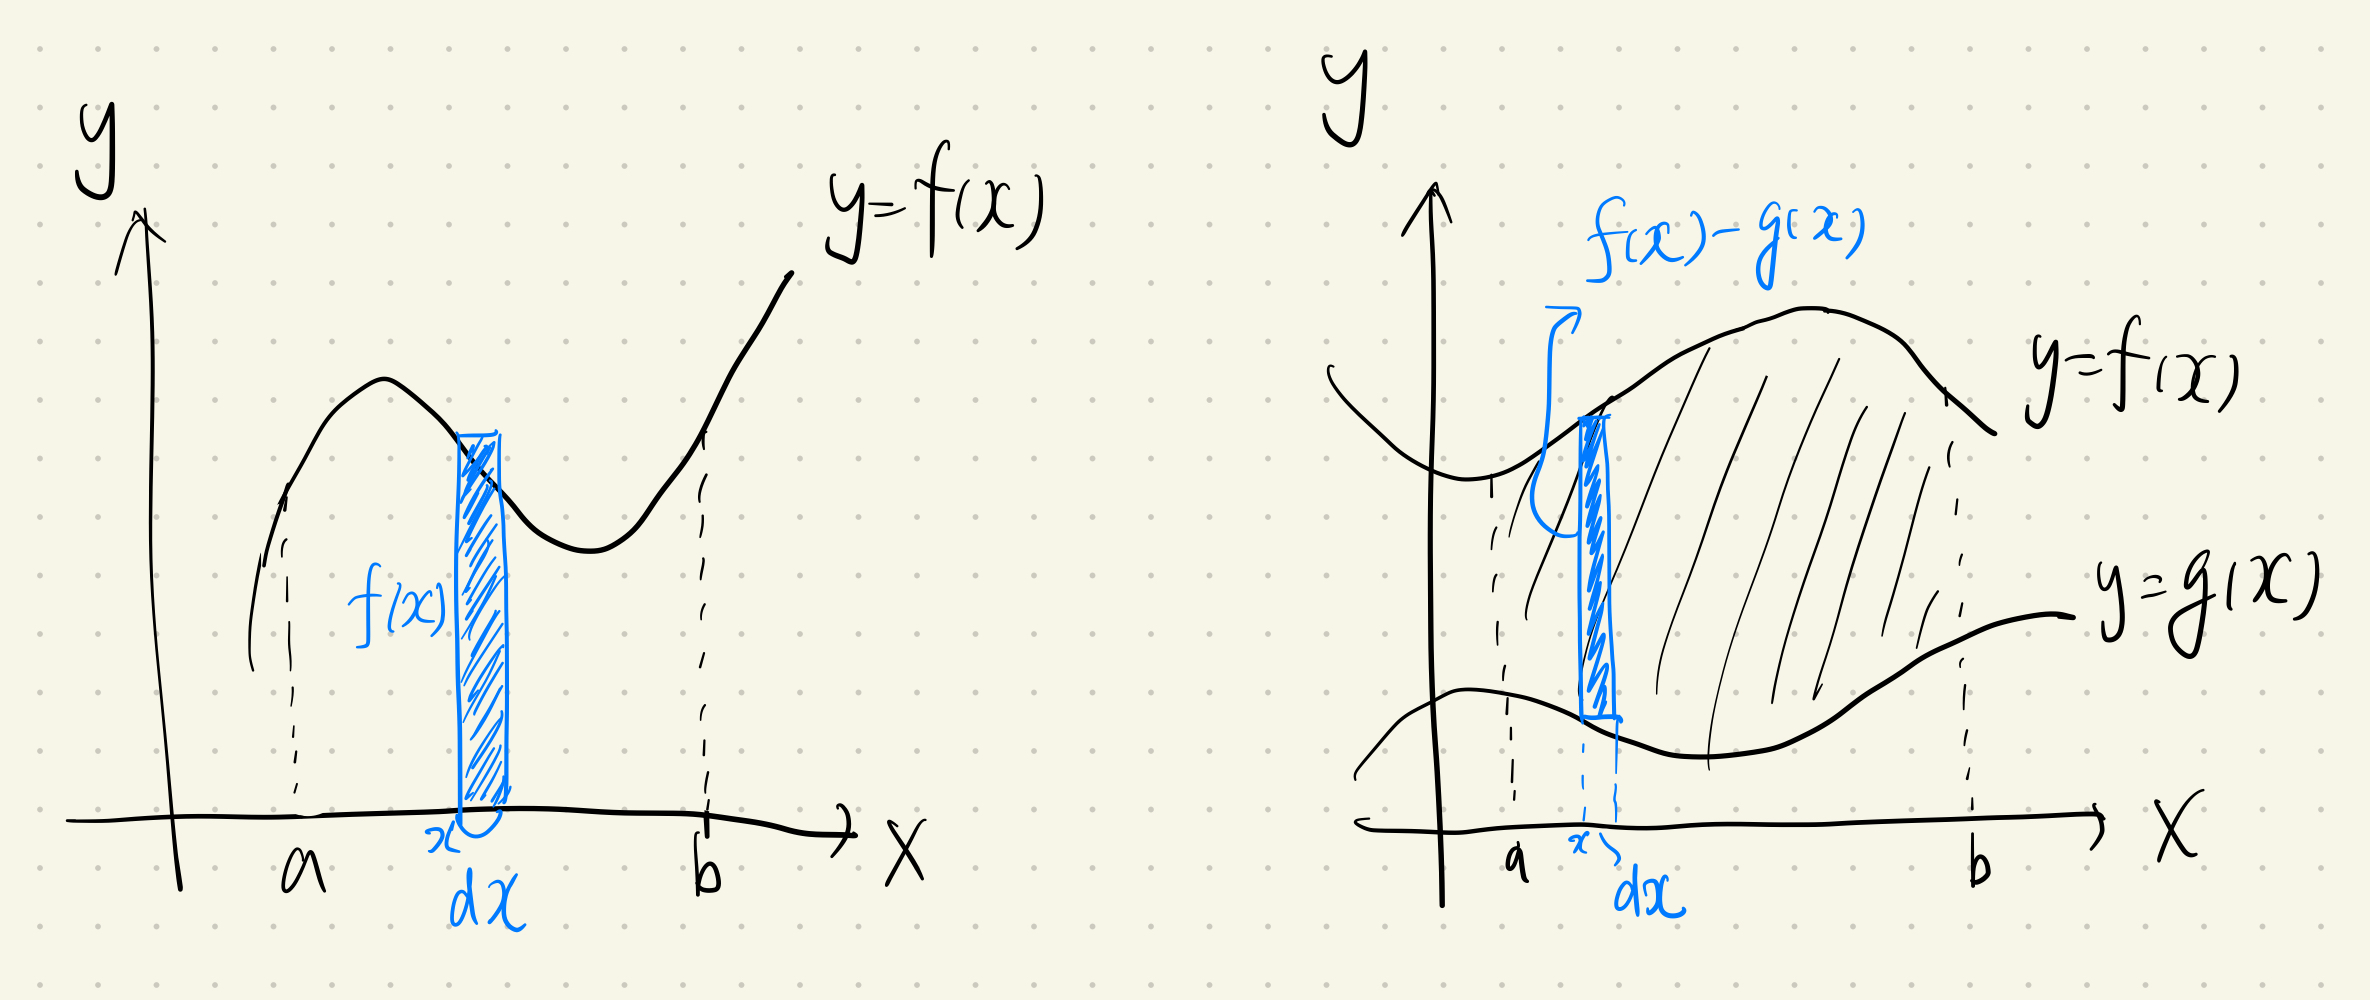
\includegraphics[width = 0.8\textwidth]{figures/chap 07/Differential_Riemann.png}
\end{figure}

This method of constructing definite integrals can be extended to the evaluation of area between the curves of two functions.  As shown in the right panel of the graph above, suppose $f(x) \ge g(x)$ within $x \in [a,b]$, and we would like to find the area enclosed by $y = f(x)$, $y = g(x)$, $x=a$ and $x=b$.  We note that the area can broken up into the sum of small shaded strips as shown in the graph, with width $dx$ and height $|f(x)-g(x)| = f(x) - g(x)$, so that the area is $(f(x)-g(x))dx$.  Since the summation ranges from $x=a$ to $x=b$, our area of interest can be written as
\[A = \int_a^b (f(x)-g(x))dx\]
Notice that in this case we are assuming that $f(x) \ge g(x)$ within $[a, b]$.  If $f(x)$ is less than $g(x)$ in any interval within $[a,b]$, then the height of the strip within that interval would be $g(x)-f(x)$, so the integrand would become $g(x)-f(x)$.  In this case, we will have to evaluate the definite integral into different parts are evaluate them separately.  We will now demonstrate its application with several examples:

\begin{eg}[]{eg: area_between_functions}
    Find the following areas using definite integrals:
    \begin{enumerate}[a)]
        \item The area between $y = (x-1)^2 + 3$ and $y = -(x-2)^2$ from $x = 1$ to $x = 3$.
        \item The area enclosed by $y = \sqrt{x}$ and $y = x^2$
        \item The area enclosed by $y = \sin x$ and $y = \cos x$ between $x = \pi/4$ to $x = 5\pi/4$
        \item The area between $y = 2x$ and $y = x^3$ from $x = -1$ to $x = 1$
    \end{enumerate}
\end{eg}

\begin{egsol}[]{egsol: area_between_functions}
    \begin{enumerate}[a)]
        \item We first graph $y = (x-1)^2 +3$ and $y = -(x-2)^2$ as follows, which shows that $(x-1)^2 +3$ is always greater than $-(x-2)^2$ between $x = 1$ and $x = 3$.  Therefore, we can directly construct the definite integral as
        \begin{align*}
            &\int_1^3 [((x-1)^2 + 3) - (-(x-2)^2)]dx\\
            =& \int_1^3 [(x^2-2x+4)+(x^2-4x+4)]dx\\
            =& \int_1^3 (2x^2-6x+8) dx\\
            =& \Big(\frac{2}{3}x^3 - 3x^2 + 8x \Big)\Big]_1^3\\
            =& \Big(\frac{2}{3}\cdot 27 - 3 \cdot 9 + 8 \cdot 3 \Big) - \Big(\frac{2}{3} - 3 + 8 \Big)\\
            =& 15 - \frac{17}{3} = \frac{28}{3} 
        \end{align*}
        \begin{center}
            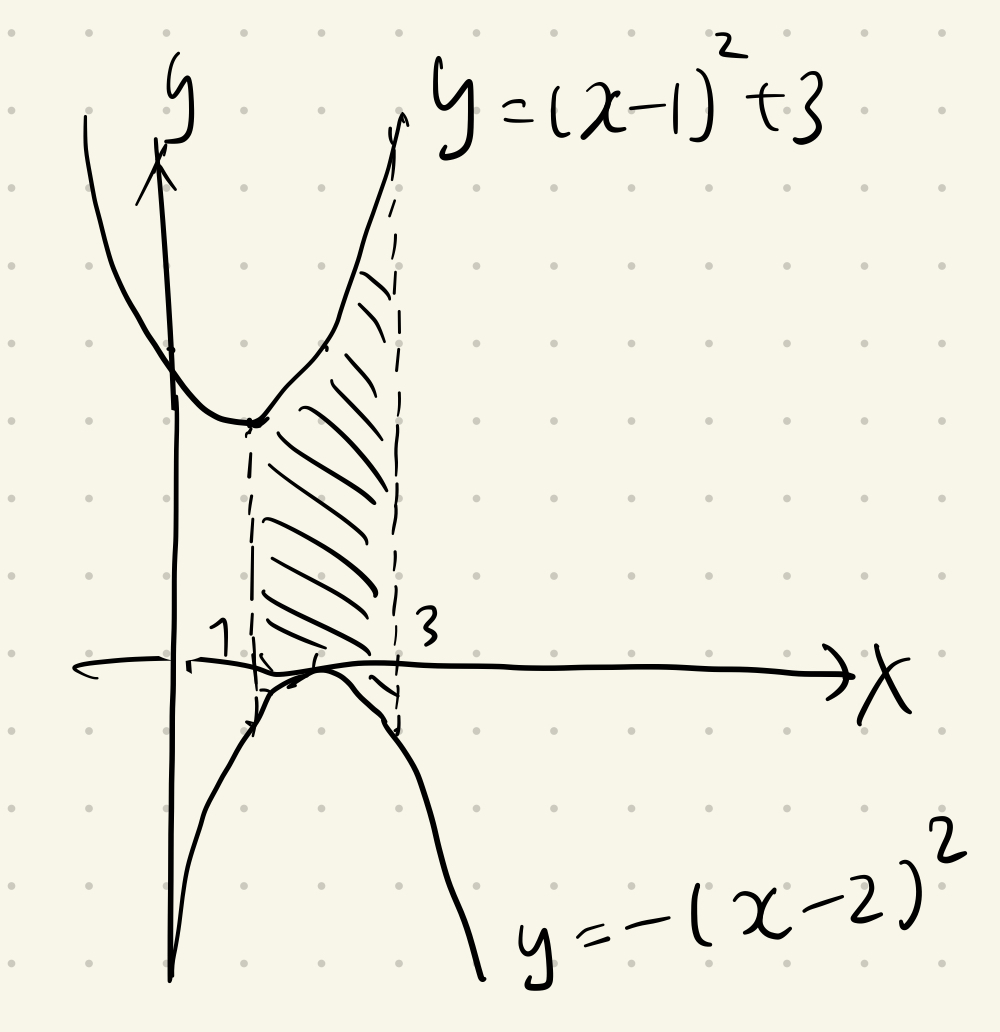
\includegraphics[width = 0.35\textwidth]{figures/chap 07/eg_7_3_a.png}
        \end{center}
        \item The problem did not give us the range of $x$ for the area enclosed by the two functions, so we first graph $y = x^2$ and $y = \sqrt{x}$.  As the following graph shows, they intersect at $(0,0)$ and $(1,1)$, and the enclosed area lies between these two points.  In addition, $\sqrt{x}$ is always no less than $x^2$ with in $x \in [0,1]$.  Therefore, we can directly construct the definite integral as
        \[\int_0^1(\sqrt{x} - x^2)~dx = \int_0^1(x^{1/2} - x^2)~dx = \Big(\frac{2}{3}x^{3/2} - \frac{1}{3}x^3\Big)\Big]_0^1 = \frac{2}{3} - \frac{1}{3} = \frac{1}{3}\]
        \begin{center}
            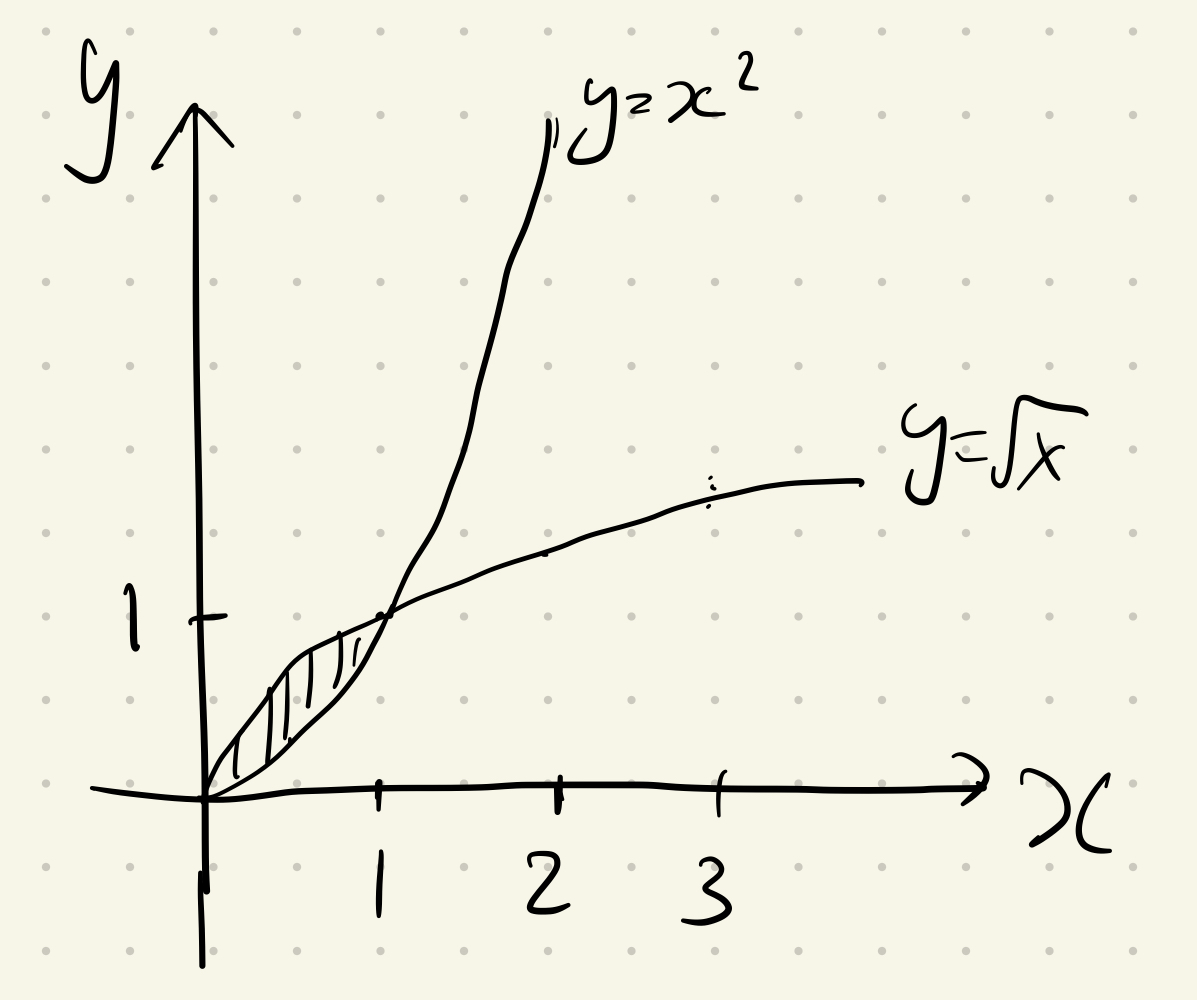
\includegraphics[width = 0.35\textwidth]{figures/chap 07/eg_7_3_b.png}
        \end{center}
        \item We first graph $y = \sin x$ and $y = \cos x$ within $x \in [\pi/4, 5\pi/4]$.  Notice that within $[\pi/4, 5\pi/4]$, we have $\sin x \ge \cos x$.  Therefore, we can directly construct the definite integral as
        \[\int_{\pi/4}^{5\pi/4} (\sin x - \cos x)~dx = (- \cos x - \sin x) \Big]_{\pi/4}^{5\pi/4} = \Big(\frac{1}{\sqrt{2}} + \frac{1}{\sqrt{2}}\Big)-\Big(-\frac{1}{\sqrt{2}} - \frac{1}{\sqrt{2}}\Big) = \frac{4}{\sqrt{2}} = 2\sqrt{2}\]
        \begin{center}
            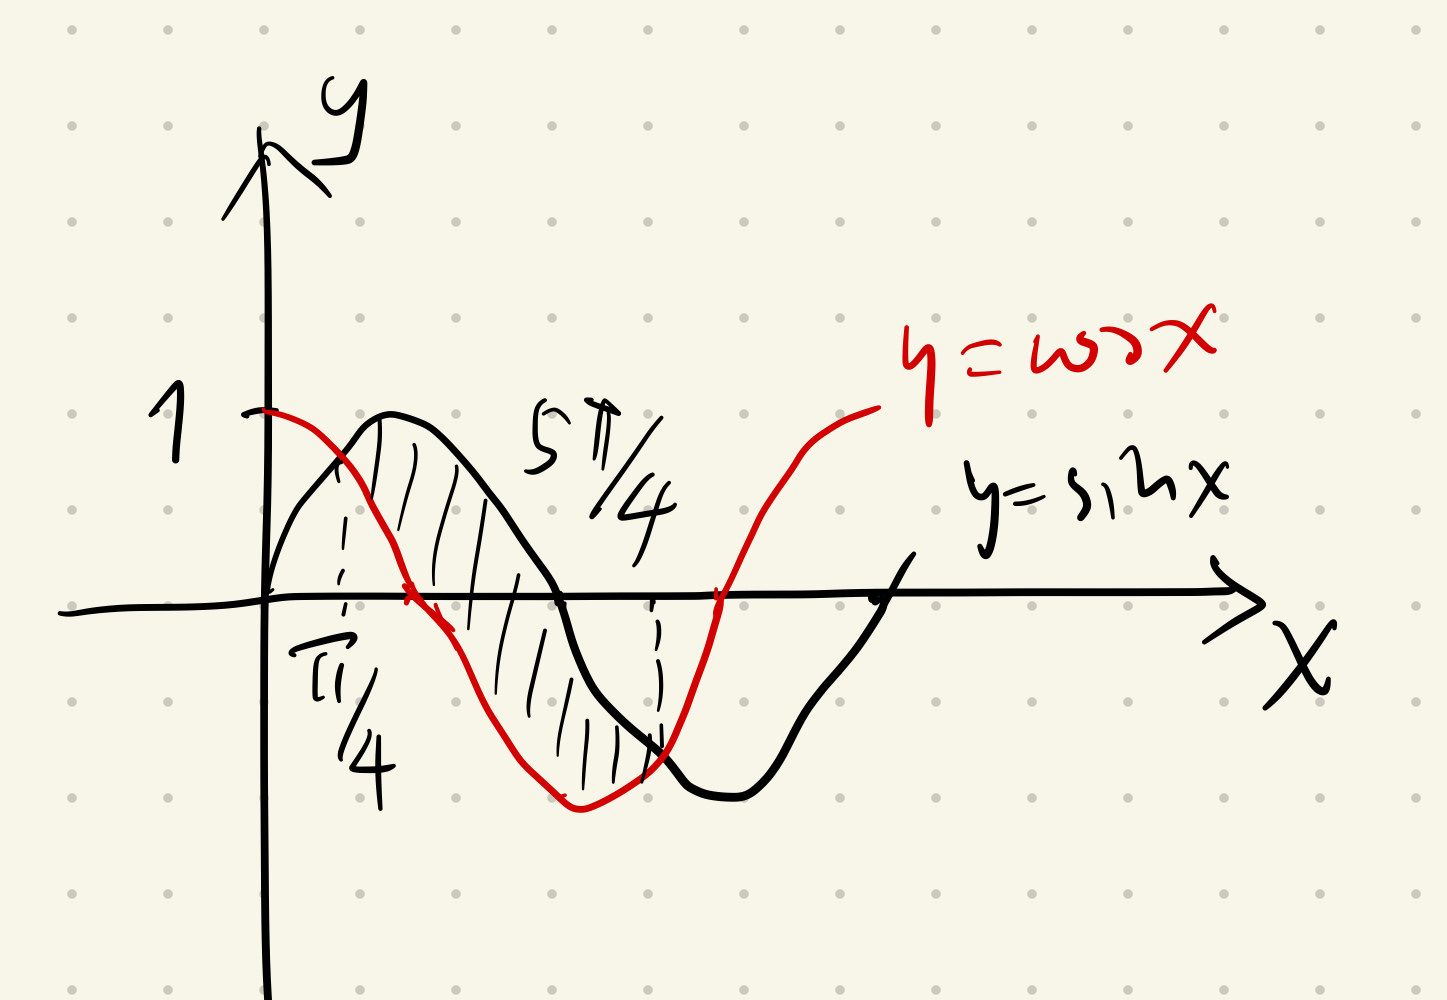
\includegraphics[width = 0.35\textwidth]{figures/chap 07/eg_7_3_c.png}
        \end{center}
        \item We first graph $y = 2x$ and $y = x^3$ within $x \in [-1, 1]$ as the follow graph, and notice that $2x > x^3$ when $x > 0$, but $x^3 > 2x$ when $x < 0$.  Therefore, we will have to construct the definite integral by splitting the range of integration into two parts, $[-1, 0]$ and $[0,1]$:
        \begin{align*}
            &\int_{-1}^0 (x^3-2x)~dx + \int_0^1 (2x-x^3)~dx\\
            =& \Big(\frac{1}{4}x^4 - x^2\Big)\Big]_{-1}^0 + \Big(x^2 - \frac{1}{4}x^4\Big)\Big]_0^1\\
            =& \Big[(0 - 0) - \Big(\frac{1}{4}-1\Big)\Big] + \Big[\Big(1 - \frac{1}{4}\Big)-(0-0)\Big] = \frac{3}{2}
        \end{align*}
        \begin{center}
            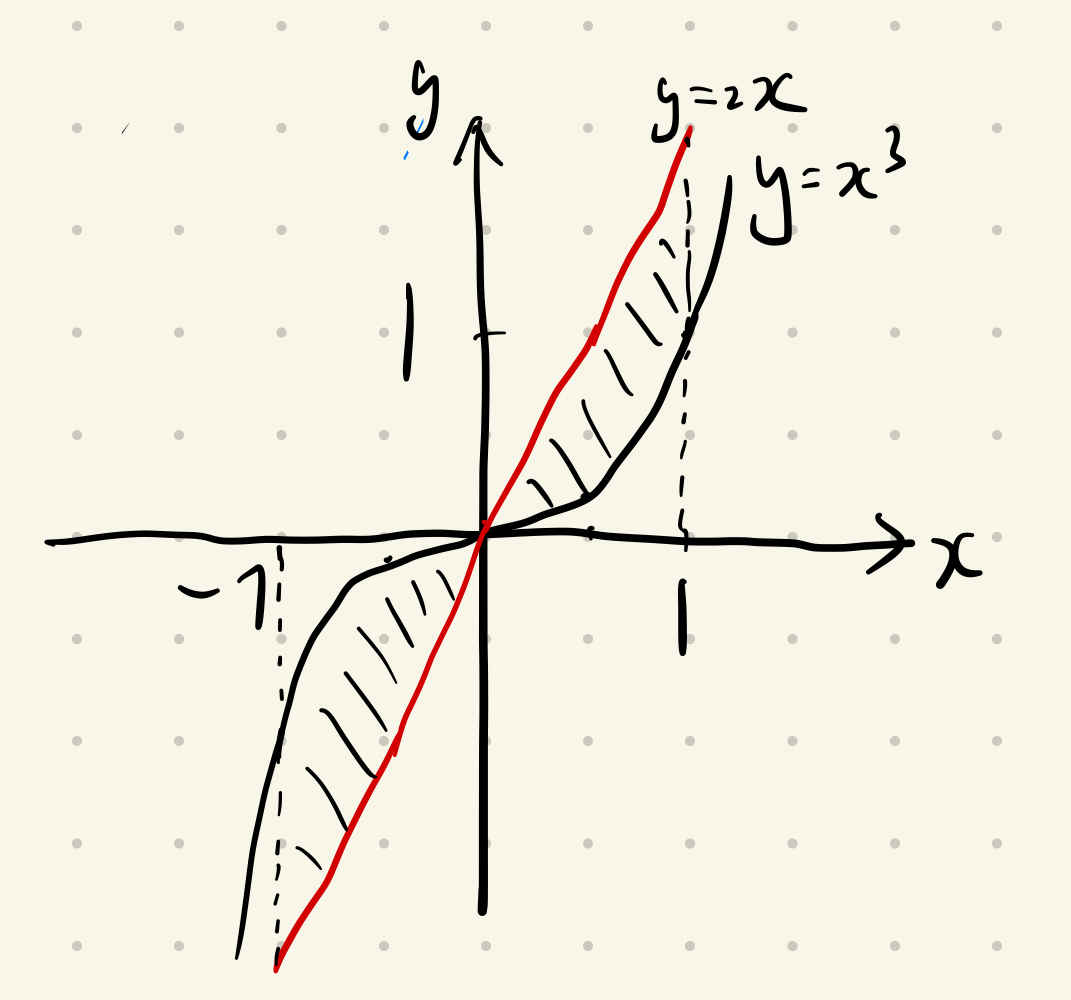
\includegraphics[width = 0.35\textwidth]{figures/chap 07/eg_7_3_d.png}
        \end{center}
        Notice that if we did not determine the order of $2x$ and $x^3$ first, and just evaluated $\int_{-1}^1 (x^3-2x)~dx$ or $\int_{-1}^1 (2x - x^3)~dx$, we would get an answer of $0$, which is clearly incorrect.
    \end{enumerate}
\end{egsol}

Apart from evaluation of areas, definite integrals can also help us find the arc length of a function, i.e. the length of its curve between two points on the curve.  To see this, lets suppose $f(x)$ is a continuous function within $x \in [a, b]$, and we wish to find the arc length of $y = f(x)$ between $(a,f(b))$ and $(b, f(b))$.  Then, we can produce the following graph:

\begin{figure}[ht]
    \centering
    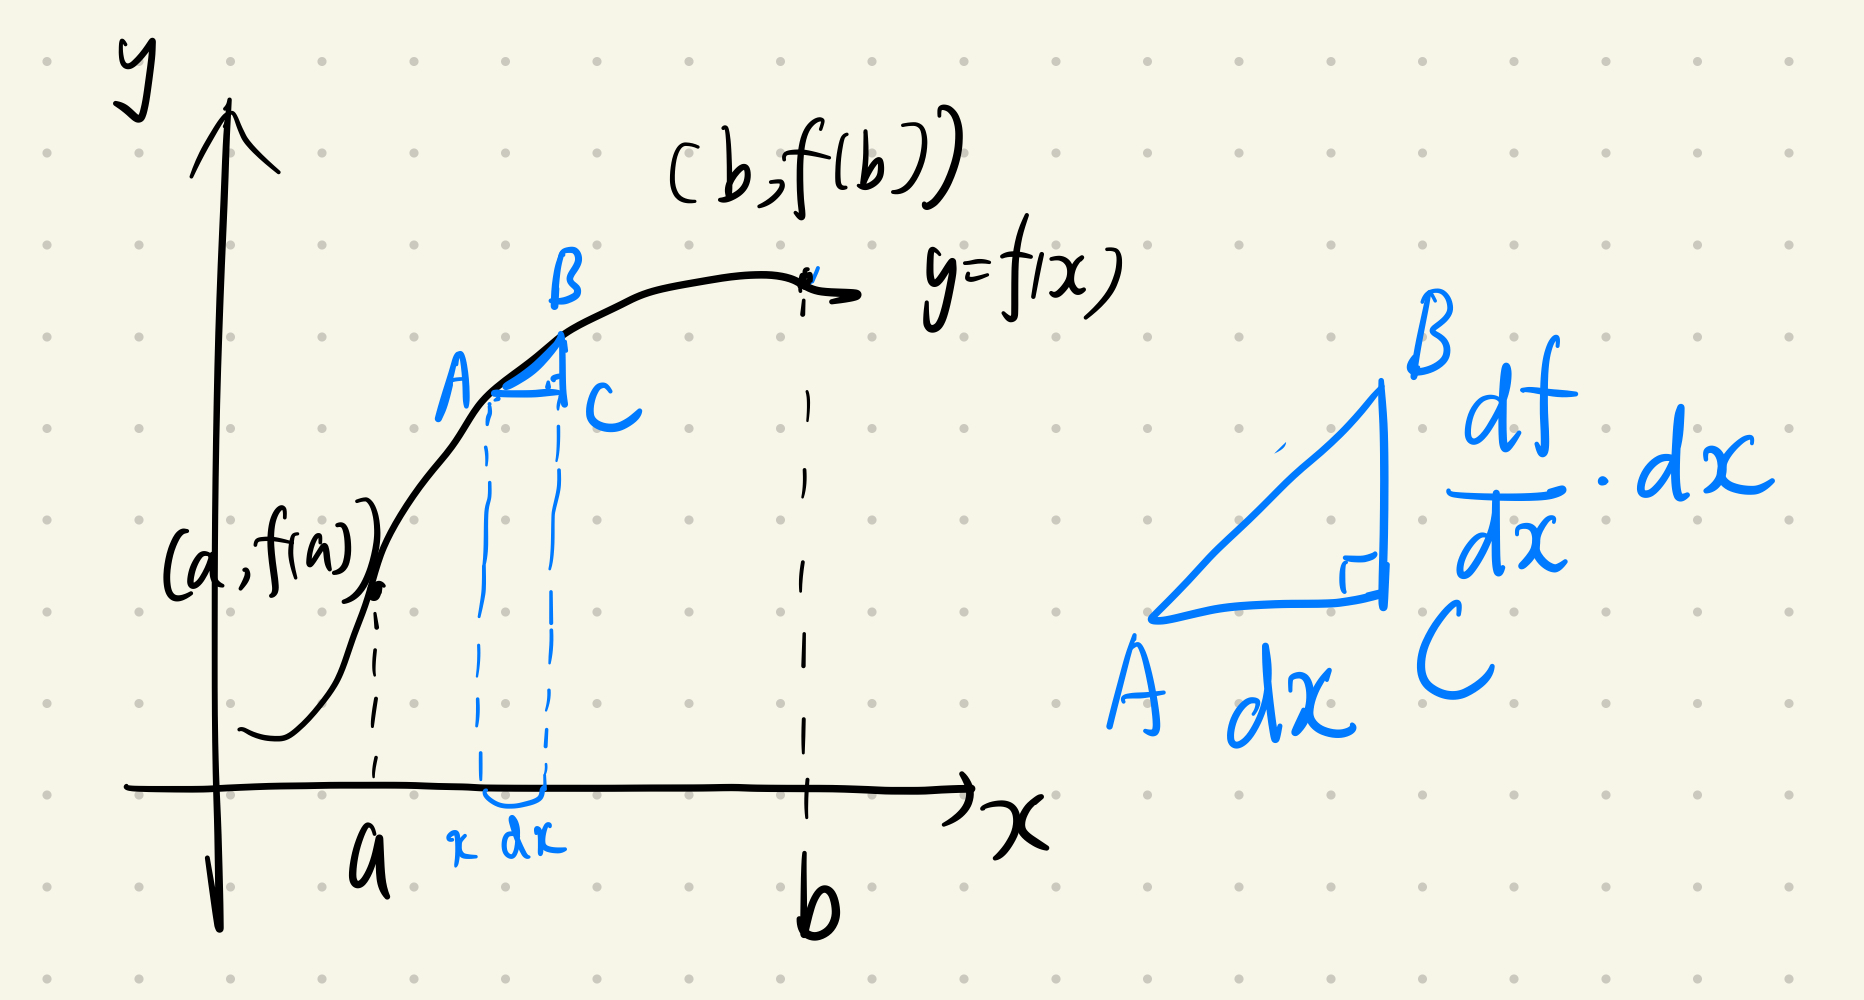
\includegraphics[width = 0.8\textwidth]{figures/chap 07/arc_length.png}
\end{figure}

As with previously where we broke up the area of interest into small strips of rectangles, here we break up the arc into small segments, shown as $\overline{AB}$ here.  As long as we can express $\overline{AB}$ as something shaped like $g(x)dx$, we can evaluate the arc length between $(a, f(a))$ and $(b, f(b))$ with the definite integral $\int_a^b g(x)~dx$.  

To find $g(x)$, we look at the right triangle $ABC$, magnified in the right panel of the graph above.  Given point $A$, point $B$ was constructed by taking an increment in $x$-coordinate by the differential $dx$, so we have $\overline{AC} = dx$.  The segment $\overline{BC}$ would then be the change in $f$ after the $x$-coordinate increment, which is the differential $df$ and can be alternatively written as $\frac{df}{dx}\cdot dx$.  Then, from the Pythagorean theorem:
\[\overline{AB} = \sqrt{\overline{AC}^2+\overline{BC}^2} = \sqrt{(dx)^2 + \Big(\frac{df}{dx}dx\Big)^2} = \sqrt{1 + \Big(\frac{df}{dx}\Big)^2}dx\]
Therefore, we have $g(x) = \sqrt{1 + \Big(\frac{df}{dx}\Big)^2}$, and the arc length is
\[S = \int_a^b \sqrt{1 + \Big(\frac{df}{dx}\Big)^2}dx\]
Let us try to evaluate a few arc lengths with our new formula:
\begin{eg}[]{eg: arc_length}
    Find the following arc lengths
    \begin{enumerate}[a)]
        \item The arc length of $y = \sqrt{1-x^2}$ between $x = -1$ and $x = 1$
        \item The arc length of $y = x^{3/2}$ between $x = 0$ and $x = 4$
        \item The arc length of $y = \ln(\sec x)$ between $x = \pi/6$ and $x = \pi/4$
    \end{enumerate}
\end{eg}

\begin{egsol}[]{egsol: arc_length}
    Find the following arc lengths
    \begin{enumerate}[a)]
        \item It is clear the $y = \sqrt{1-x^2}$ is the upper half of a circle centered at the origin with radius $1$, so our arc length should be half the circumference of a circle of radius $1$, which is $\pi$.  We can verify this by noting $\frac{dy}{dx} = -\frac{x}{\sqrt{1-x^2}}$, so the arc length should be
        \begin{align*}
            S &= \int_{-1}^1 \sqrt{1+\Big(\frac{dy}{dx}\Big)^2}~dx\\
            &= \int_{-1}^1 \sqrt{1+\Big(-\frac{x}{\sqrt{1-x^2}}\Big)^2}~dx\\
            &= \int_{-1}^1 \frac{1}{\sqrt{1-x^2}}~dx\\
            &= \arcsin x\Big]_{-1}^1 = \frac{\pi}{2} - \Big(-\frac{\pi}{2}\Big) = \pi
        \end{align*}
        where is identical to what we have predicted.
        \item Since $\frac{dy}{dx} = \frac{d x^{3/2}}{dx} = \frac{3}{2} \sqrt{x}$, the arc length can be evaluated by
        \begin{align*}
            S &= \int_0^4\sqrt{1+\Big(\frac{dy}{dx}\Big)^2}~dx\\
            &= \int_0^4\sqrt{1+\big(\frac{3}{2}\sqrt{x}\big)^2}~dx\\
            &= \int_0^4\sqrt{1+\frac{9}{4}x}~dx
        \end{align*}
        Now let $u = 1+\frac{9}{4}x$, so that $du = \frac{9}{4}dx$.  In addition, for the integration limits, when $x = 4$, $u = 10$; when $x = 0$, $u = 1$.  Therefore we have
        \begin{align*}
            S &= \int_0^4\sqrt{1+\frac{9}{4}x}~dx\\
            &=\frac{4}{9} \int_0^4\sqrt{1+\frac{9}{4}x}~\Big(\frac{9}{4}dx\Big)\\
            &=\frac{4}{9}  \int_1^{10}\sqrt{u}~du\\
            &= \frac{4}{9}\cdot \frac{2}{3}u^{3/2}\Big]_1^{10} = \frac{8}{27}(10\sqrt{10}-1)
        \end{align*}
        \item Since $\frac{dy}{dx} = \frac{d \ln(\sec x)}{dx} = \tan x$, the arc length can be evaluated by
        \begin{align*}
            S &= \int_{\pi/6}^{\pi/4}\sqrt{1+\Big(\frac{dy}{dx}\Big)^2}~dx\\
            &= \int_{\pi/6}^{\pi/4}\sqrt{1+\tan^2 x}~dx\\
            &= \int_{\pi/6}^{\pi/4} \sec x~dx\\
            &= \ln|\sec x + \tan x|\big]_{\pi/6}^{\pi/4}\\
            &= \ln|\sqrt{2} + 1| - \ln\Big|\frac{2}{\sqrt{3}}+\frac{1}{\sqrt{3}}\Big| = \ln \frac{\sqrt{2}+1}{\sqrt{3}}
        \end{align*}
    \end{enumerate}
\end{egsol}

\begin{ex}[]{ex: arc_length}
    Find the arc length of $y = x^2$ between $x = 0$ and $x = 1/2$
\end{ex}

\begin{exsol}[]{exsol: arc_length}
    Since $\frac{dy}{dx} = \frac{dx^2}{dx} = 2x$, the arc length can be evaluated by
    \[S = \int_0^{1/2} \sqrt{1+\Big(\frac{dy}{dx}\Big)^2}~dx = \int_0^{1/2} \sqrt{1+(2x)^2}~dx\]
    To eliminate the square root, we let $2x = \tan \theta$, so that $dx = \frac{1}{2}\sec^2 \theta d \theta$.  For the limits of integration, when $x = 1/2$, $\theta = \arctan 1 = \frac{\pi}{4}$; when $x = 0$, $\theta = \arctan 0 = 0$.  Therefore we have
    \[S = \int_0^{1/2} \sqrt{1+(2x)^2}~dx = \int_0^{\pi/4} \sqrt{1+\tan^2\theta}~\frac{1}{2}\sec^2\theta d\theta= \frac{1}{2} \int_0^{\pi/4} \sec^3\theta d\theta\]
    To evaluate $\int_0^{\pi/4} \sec^3\theta d\theta$, we will need to use integration by parts where $u = \sec \theta, dv/d\theta = \sec^2 \theta$, so that $du/dx = \sec\theta \tan\theta, v = \tan \theta$:
    \begin{align*}
        \int_0^{\pi/4} \sec^3\theta d\theta &= \int_0^{\pi/4} \sec \theta \cdot \sec^2 \theta~d\theta\\
        &= \sec \theta \tan \theta\big]_0^{\pi/4} - \int_0^{\pi/4} \sec\theta \tan\theta \cdot \tan\theta d\theta\\
        &= \sec \theta \tan \theta\big]_0^{\pi/4} - \int_0^{\pi/4} \sec\theta \tan^2\theta d\theta\\
        &= \sec \theta \tan \theta\big]_0^{\pi/4} - \int_0^{\pi/4} \sec\theta (\sec^2\theta -1) d\theta\\
        &= \sec \theta \tan \theta\big]_0^{\pi/4} - \int_0^{\pi/4} \sec^3\theta d\theta + \int_0^{\pi/4} \sec\theta~d\theta\\
        &= \sec \theta \tan \theta\big]_0^{\pi/4} + \ln|\sec\theta + \tan\theta|\big]_0^{\pi/4} - \int_0^{\pi/4} \sec^3\theta d\theta\\
    \end{align*}
    Now both sides of the equation has the definite integral of $\int_0^{\pi/4}\sec^3\theta~d\theta$, so we aggregate them to the left:
    \begin{align*}
        &2\int_0^{\pi/4}\sec^3\theta~d\theta\\
        = &\Big(\sec\frac{\pi}{4}\tan\frac{\pi}{4}-\sec 0 \tan 0\Big) + \Big(\ln|\sec\frac{\pi}{4}+\tan\frac{\pi}{4}|-\ln|\sec 0 + \tan 0|\Big)\\
        = & (\sqrt{2} -0)+ (\ln|\sqrt{2}+1|-\ln|1|) = \sqrt{2}+\ln(\sqrt{2}+1)
    \end{align*}
    Therefore, we have
    \[ S= \frac{1}{2}\int_0^{\pi/4}\sec^3\theta~d\theta = \frac{1}{4} \cdot 2\int_0^{\pi/4}\sec^3\theta~d\theta = \frac{1}{4}[\sqrt{2}+\ln(\sqrt{2}+1)]\]
\end{exsol}

\section{Volume and surface area for solids of revolution}

In the previous section we've seen that definite integrals can help us evaluate the area under the curve, area between two curves, and the arc length of a curve.  We arrived at these definite integrals by slicing the area or arc length into pieces that can be expressed with $g(x)dx$, and then integrating them back to obtain the area or arc length of interest.  In this section, we will show that definite integrals can also help us evaluate the volume and surface area for solids of revolution, which are solids that has at least one axis of rotational symmetry, eg. a ball, an ellipsoid or a cone. 

Suppose a solid of revolution can be created by taking a curve $y = f(x)$ from $x = a$ to $x = b$ and rotating it about the $x$-axis.  For example, in the following graph, we have a clay pot-shaped solid that is rotationally symmetric along the $x$-axis.  Then, analogous to our previous approach, to evaluate the volume of the solid, we can slice the solid along the $x$-axis to get a series of thin disks.  If the volume of these disks can be expressed in the form of $g(x)dx$, then we can integrate $g(x)$ along the $x$-axis from $x=a$ to $x=b$ to get our desired volume.  

\begin{figure}[ht]
    \centering
    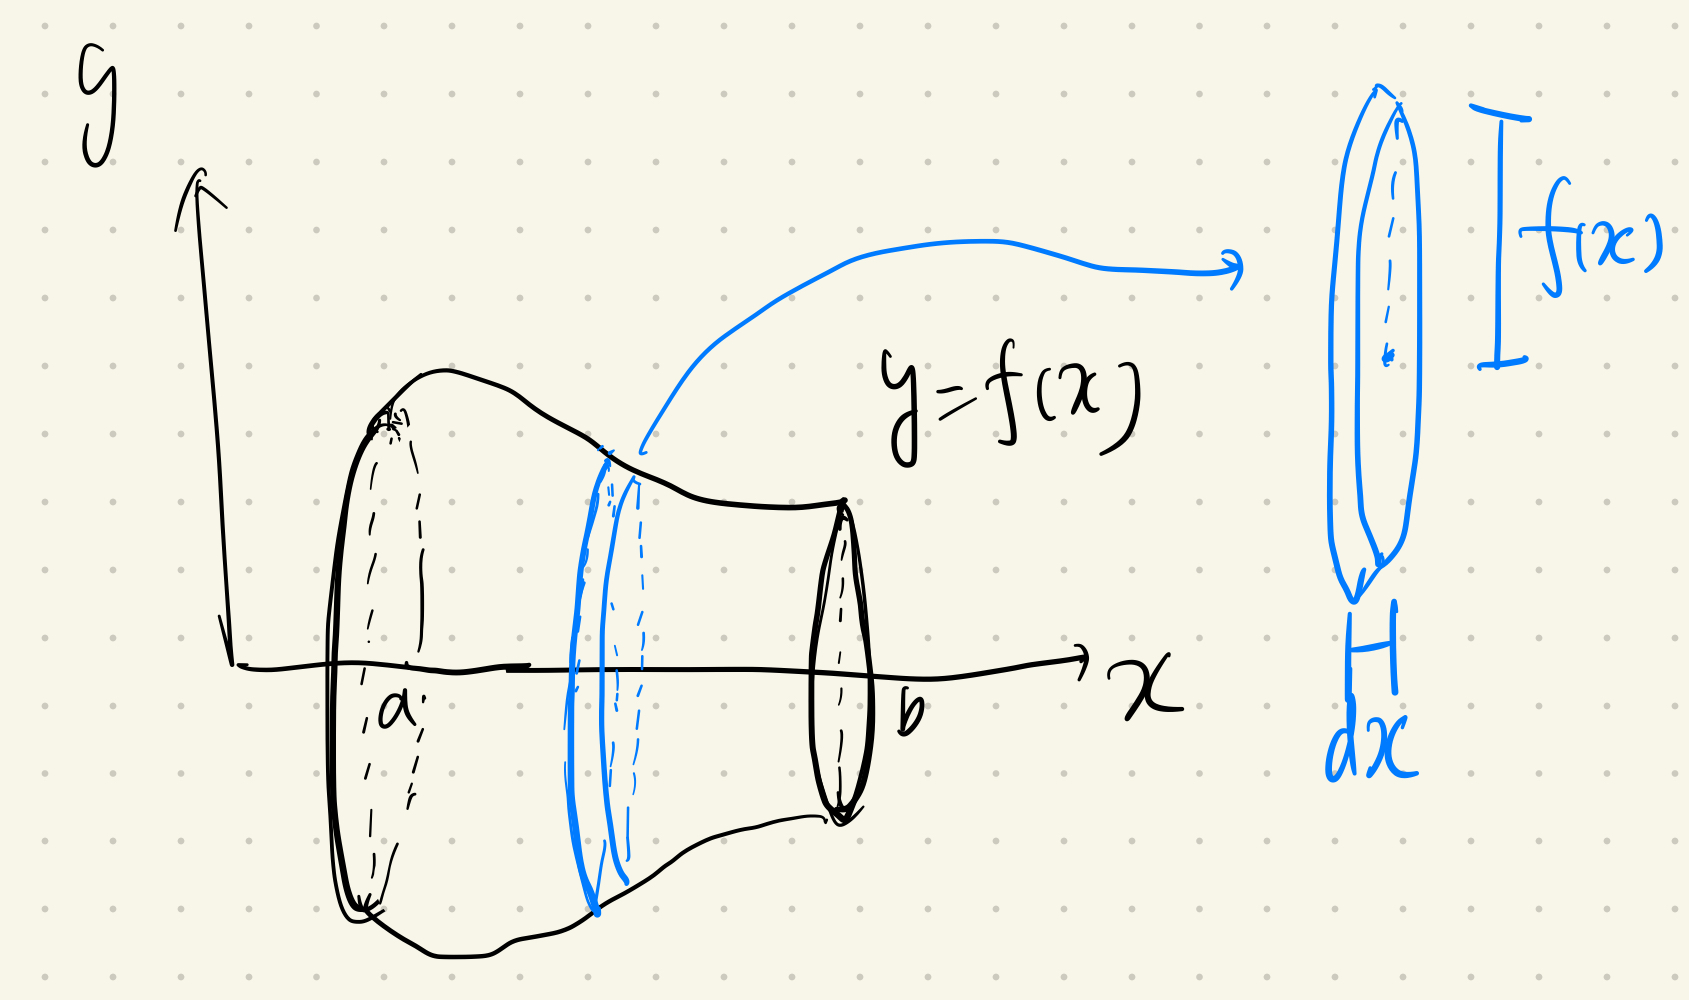
\includegraphics[width = 0.6\textwidth]{figures/chap 07/revolution_vol.png}
\end{figure}

The right panel of the graph above shows one slice of the thin disk.  As the disk gets thinner and thinner, it is approaching the shape of the cylinder.  Therefore, to evaluate the volume of the disk, we need to know the area of its base and its width.  For the width, since we are slicing along the $x$-axis, the width of the disk would be the differential $dx$.  For the area of its base, since this is a rotational solid, the section of each disk would be a circle, with its radius as $f(x)$ since we are rotating $y = f(x)$ around the $x$-axis.  Therefore, the area of the base should be $\pi (f(x))^2$, and the volume of the disk is then $\pi (f(x))^2 dx$.  At last, the volume for the solid of revolution would be
\[V = \int_a^b \pi (f(x))^2~dx\]

\begin{figure}[ht]
    \centering
    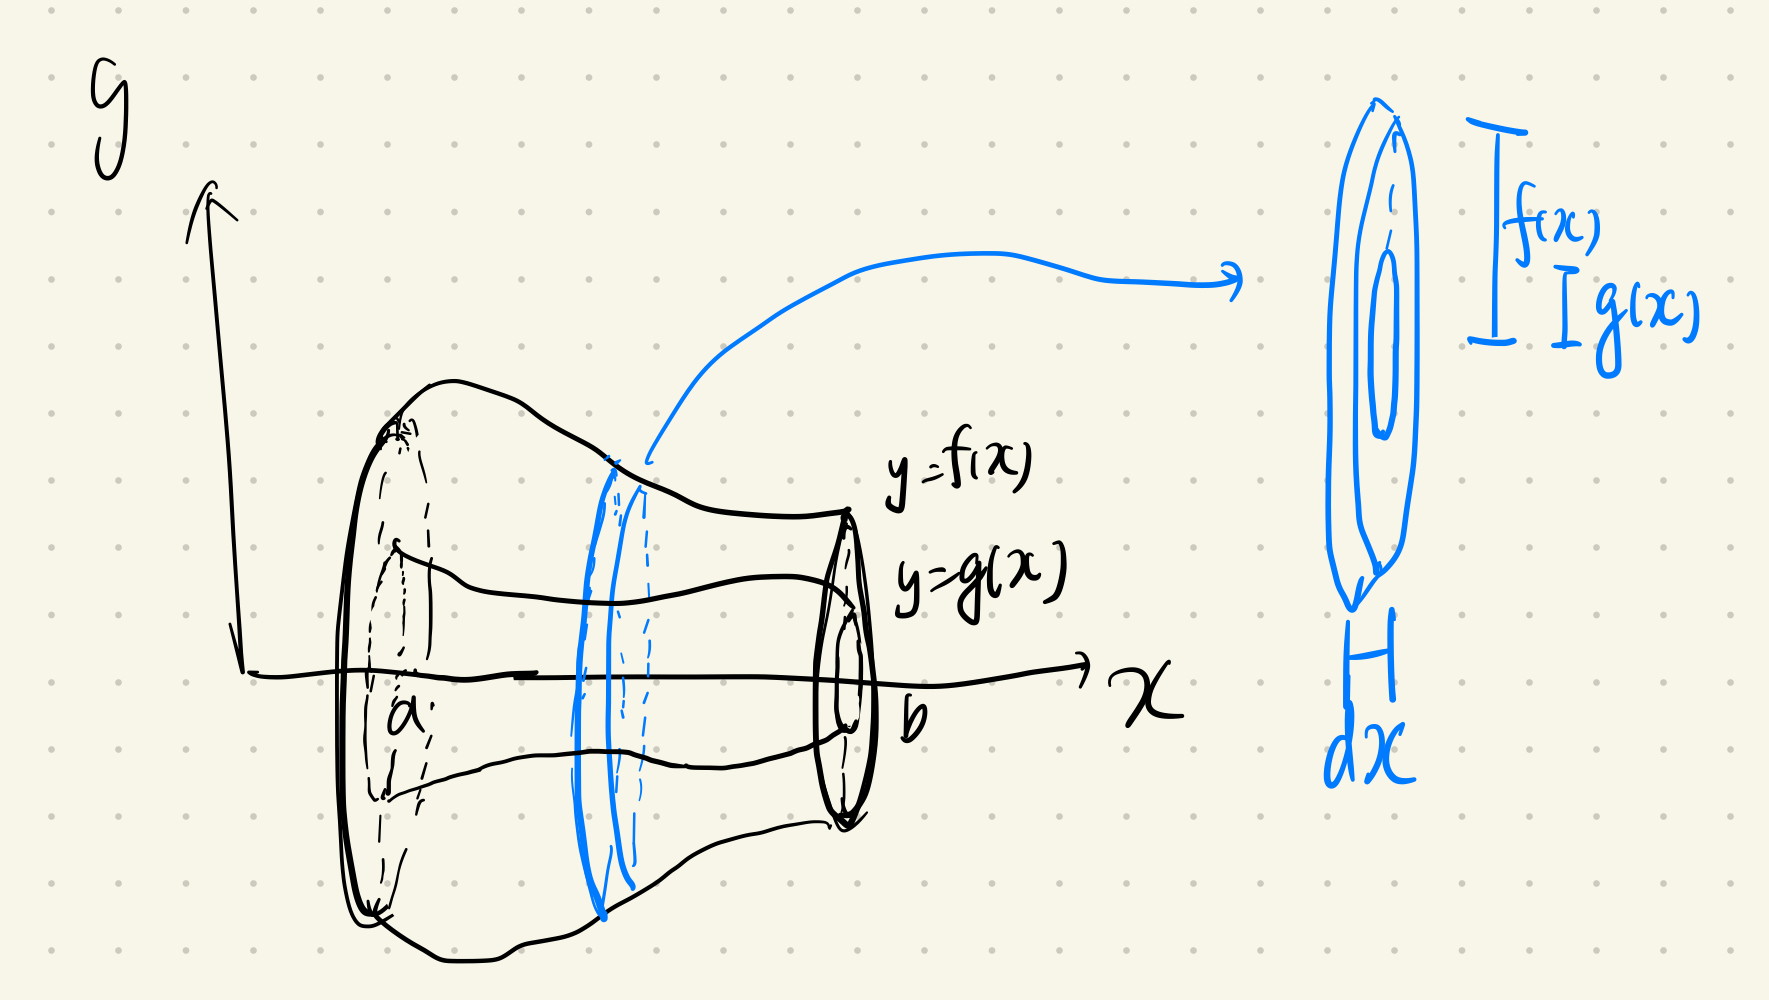
\includegraphics[width = 0.6\textwidth]{figures/chap 07/revolution_vol_ring.png}
\end{figure}

In the case where the solid revolution is formed by rotating the area between two curves along the $x$-axis, such as the graph above where the area between $y=f(x)$ and $y=g(x)$ are rotated, then volume of the thin disks, which is now a thing ring, would be $\pi [(f(x))^2-(g(x))^2] dx$ instead since we have to subtract the volume of the inner cylinder from the outer cylinder.  Therefore, the volume for the hallow solid of revolution would be 
\[V = \int_a^b \pi [(f(x))^2-(g(x))^2]~dx\]

Here our method slices the solid of revolution into disks or rings, depending on if the solid is hallow inside.  Therefore, this method is sometimes termed as the \textit{method of disks} or \textit{method of rings}.  We now show how they work with some examples:

\begin{eg}[]{eg: rev_solid_vol_ring}
    Verify the volume of the following solids using the method of disks
    \begin{enumerate}[a)]
        \item A ball of radius $r$ has volume $\frac{4}{3}\pi r^3$.
        \item A cone of height $h$ and radius of base $r$ has volume $\frac{1}{3}\pi r^2 h$.
    \end{enumerate}
\end{eg}

\begin{egsol}[]{egsol: rev_solid_vol_ring}
    \begin{enumerate}[a)]
        \item If we put a semi-circle of radius $r$ on the $x$-axis and rotate it about the axis, then we would get a ball of radius $r$ as the solid of revolution.  Therefore, as shown in the graph below, we can let $y = f(x) = \sqrt{r^2-x^2}$, which represents a semi-circle of radius $r$ with center at the origin, and evaluate the volume for the solid of revolution from $x = -r$ to $x = r$, which yields
        \begin{center}
            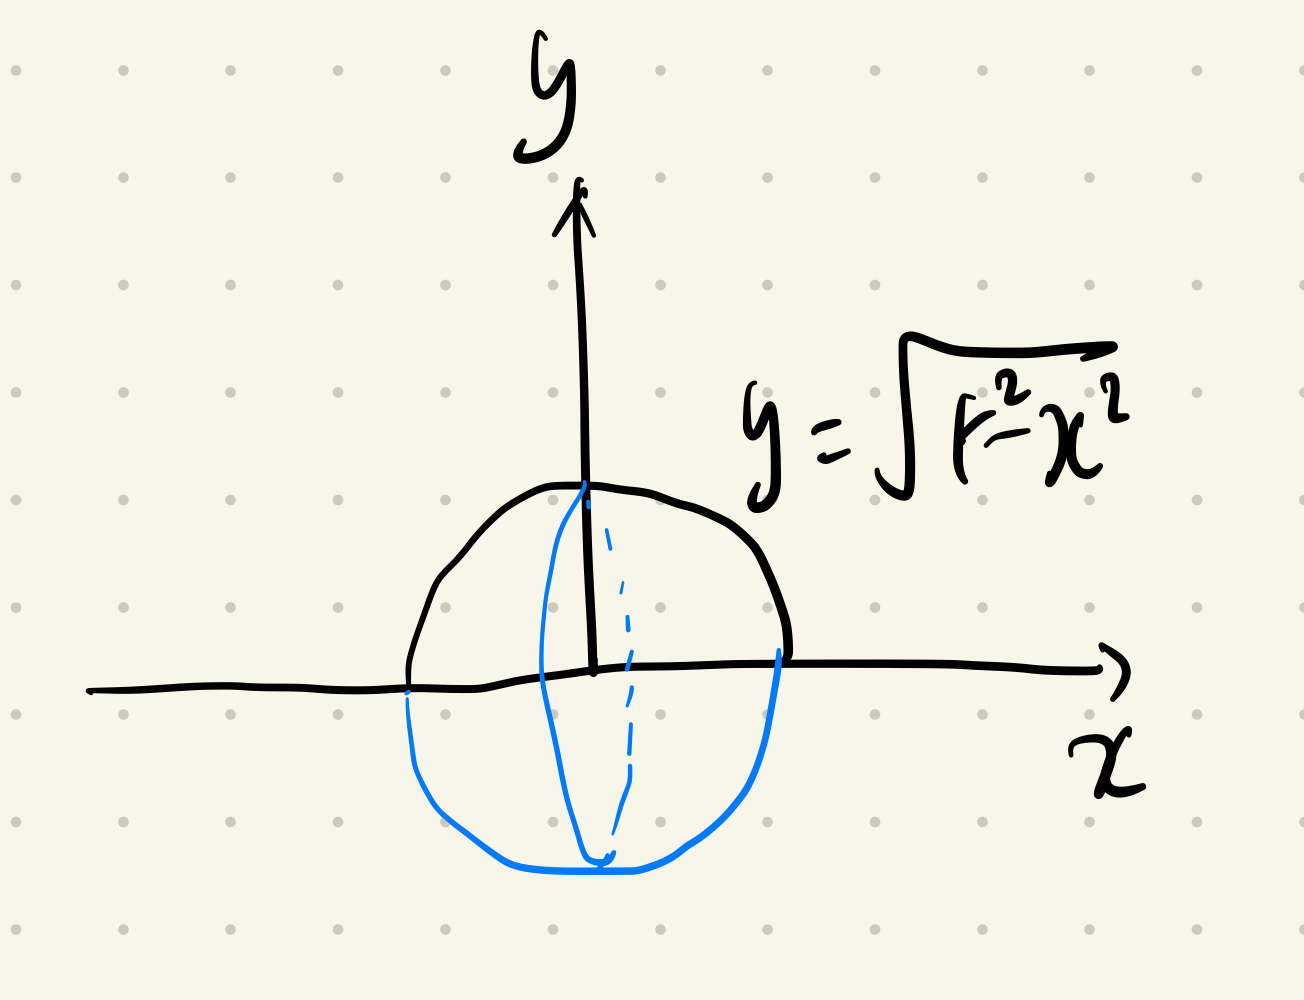
\includegraphics[width = 0.3\textwidth]{figures/chap 07/rev_solid_ball.png}
        \end{center}
        \begin{align*}
            V &= \int_{-r}^r \pi (\sqrt{r^2-x^2})^2~dx\\
            &= \int_{-r}^r (\pi r^2 - \pi x^2) ~dx\\
            &= \pi r^2 x - \frac{1}{3} \pi x^3\big]{-r}^r\\
            &= (\pi r^2 \cdot r - \frac{1}{3} \pi r^3) - ((\pi r^2 \cdot (-r) - \frac{1}{3} \pi (-r)^3))\\
            &= \big(1-\frac{1}{3} + 1 - \frac{1}{3}\big)r^3 = \frac{4}{3}\pi r^3
        \end{align*}
        \item As shown in the following graph, if we rotate a right angle triangle with base $h$ and height $r$ about the $x$-axis, we would get a cone described by the problem.  The hypotenuse of the triangle would have a slope of $r/h$, so its equation would be $y = (r/h)x$.  We can thus evaluate the volume for the solid of revolution from $x = 0$ to $x = h$ for $y = (r/h) x$, which yields
        \begin{center}
            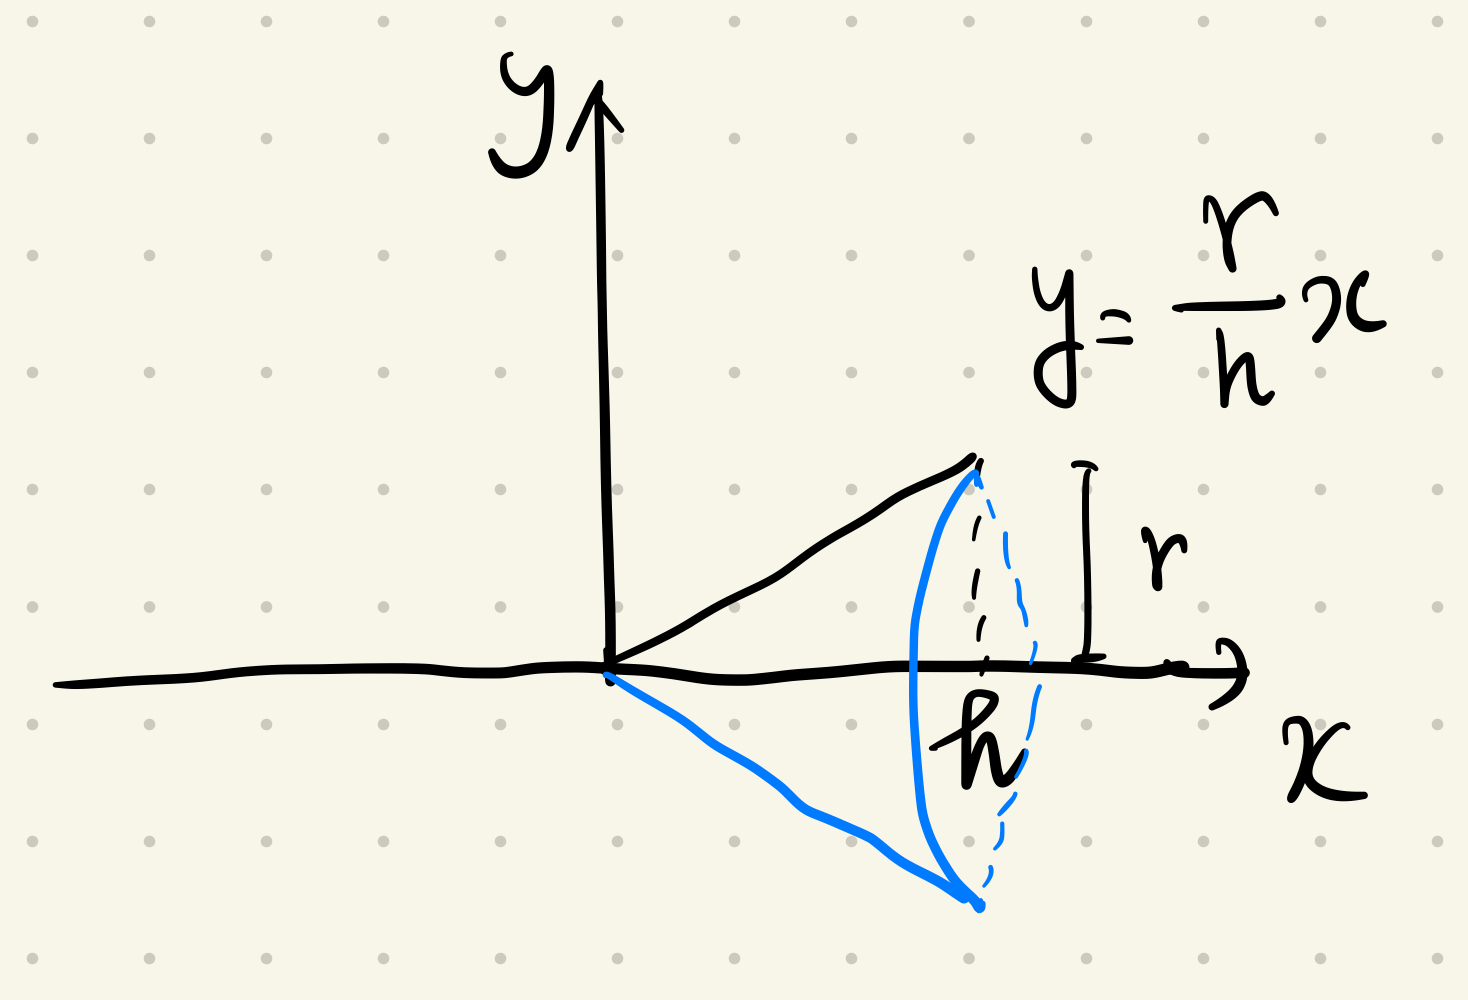
\includegraphics[width = 0.3\textwidth]{figures/chap 07/rev_solid_cone.png}
        \end{center}
        \begin{align*}
            V &= \int_0^h \pi \big(\frac{r}{h}x)^2~dx\\
            &= \int_0^h \pi \frac{r^2}{h^2} x^2~dx\\
            &= \pi \frac{r^2}{h^2} \cdot \frac{1}{3}x^3 \Big]_0^h\\
            &= \pi \frac{r^2}{h^2} \cdot \frac{1}{3}h^3 = \frac{1}{3} \pi r^2 h
        \end{align*}
    \end{enumerate}
\end{egsol}

\begin{ex}[]{ex: rev_solid_vol_ring}
    Find the volume of the solid constructed by revolving the area enclosed by $y = x$ and $y = \sqrt{x}$ around the $x$-axis.
\end{ex}

\begin{exsol}[]{exsol: rev_solid_vol_ring}
    \begin{center}
        \includegraphicsex{width = 0.65\textwidth, draft}{width = 0.65\textwidth}{figures/chap 07/method_of_rings.png}
    \end{center}
    As shown in the graph above, the range of $x$-coordinate for the area enclosed by $y=x$ and $y=\sqrt{x}$ is $x=0$ to $x=1$.  When this area is revolved around the axis to form a solid of revolution, we can slice the solid along the $x$-axis and get rings shaped as the right hand side, with width $dx$ and area of the base made up of two concentric circles, the larger one with radius $\sqrt{x}$ (since $\sqrt{x} \ge x$ within $x \in [0, 1]$) and the smaller one with radius $x$.  Therefore, the ring slice has volume
    \[\pi [(\sqrt{x})^2 - x^2] dx = \pi (x - x^2) dx\]
    and the volume the whole solid can be found by integrating the volume of the ring slices and letting $x$ go from $0$ to $1$:
    \[\int_0^1 \pi (x - x^2) dx = \pi \int_0^1 (x - x^2) dx = \pi \Big(\frac{1}{2}x^2 - \frac{1}{3}x^3\Big)\Big]_0^1 = \pi \Big(\frac{1}{2}-\frac{1}{3}) = \frac{\pi}{6}\]
\end{exsol}

\begin{ex}[]{ex: rev_solid_vol_y}
    Find the volume of the solid constructed by revolving the area between the $y$-axis and the curve of $y = x^2$ from $x = 0$ to $x = 2$ around the $y$-axis. 
\end{ex}

\begin{exsol}[]{exsol: rev_solid_vol_y}
    \begin{center}
        \includegraphicsex{width = 0.6\textwidth, draft}{width = 0.6\textwidth}{figures/chap 07/method_of_disks_y.png}
    \end{center}
    In this problem, the solid of revolution is not revolving about the $x$-axis but instead the $y$-axis, so we cannot directly use the formula shown in the previous text.  However, we can still use the method of disks, but now as shown in the graph, we need to slice the solid of revolution along the $y$-axis instead of the $x$-axis to get slices of disks shaped as shown on the right.  The height of the disk would be $dy$, and when the $y$-coordinate of the disk is denoted as $y$, the radius of the disk would be $\sqrt{y}$ since $(\sqrt{y}, y)$ would be on the curve.  Therefore, the volume of the slice of disk is
    \[\pi (\sqrt{y})^2 dy = \pi y~dy\]
    and the volume of the whole solid can be evaluated by integrating the volume of the disks from $y = 0^2 = 0$ to $y = 2^2 = 4$
    \[\int_0^4 \pi y~dy = \pi \int_0^4 y~dy = \pi \Big(\frac{1}{2}y^2\Big)\Big]_0^4 = \frac{1}{2}\cdot 16 = 8\]
\end{exsol}

In the previous exercise, we found the volume of a solid revolving about the $y$-axis with the method of disks.  This approach worked since we could express the radius of each disk with $y$ by solving for $x$ in $y = x^2$.  However, in the case where the curve revolving the $y$-axis is more complex, eg. $y =  e^x - x$, we cannot solve for $x$ anymore, so the method of disks does not work.

\begin{figure}[ht]
    \centering
    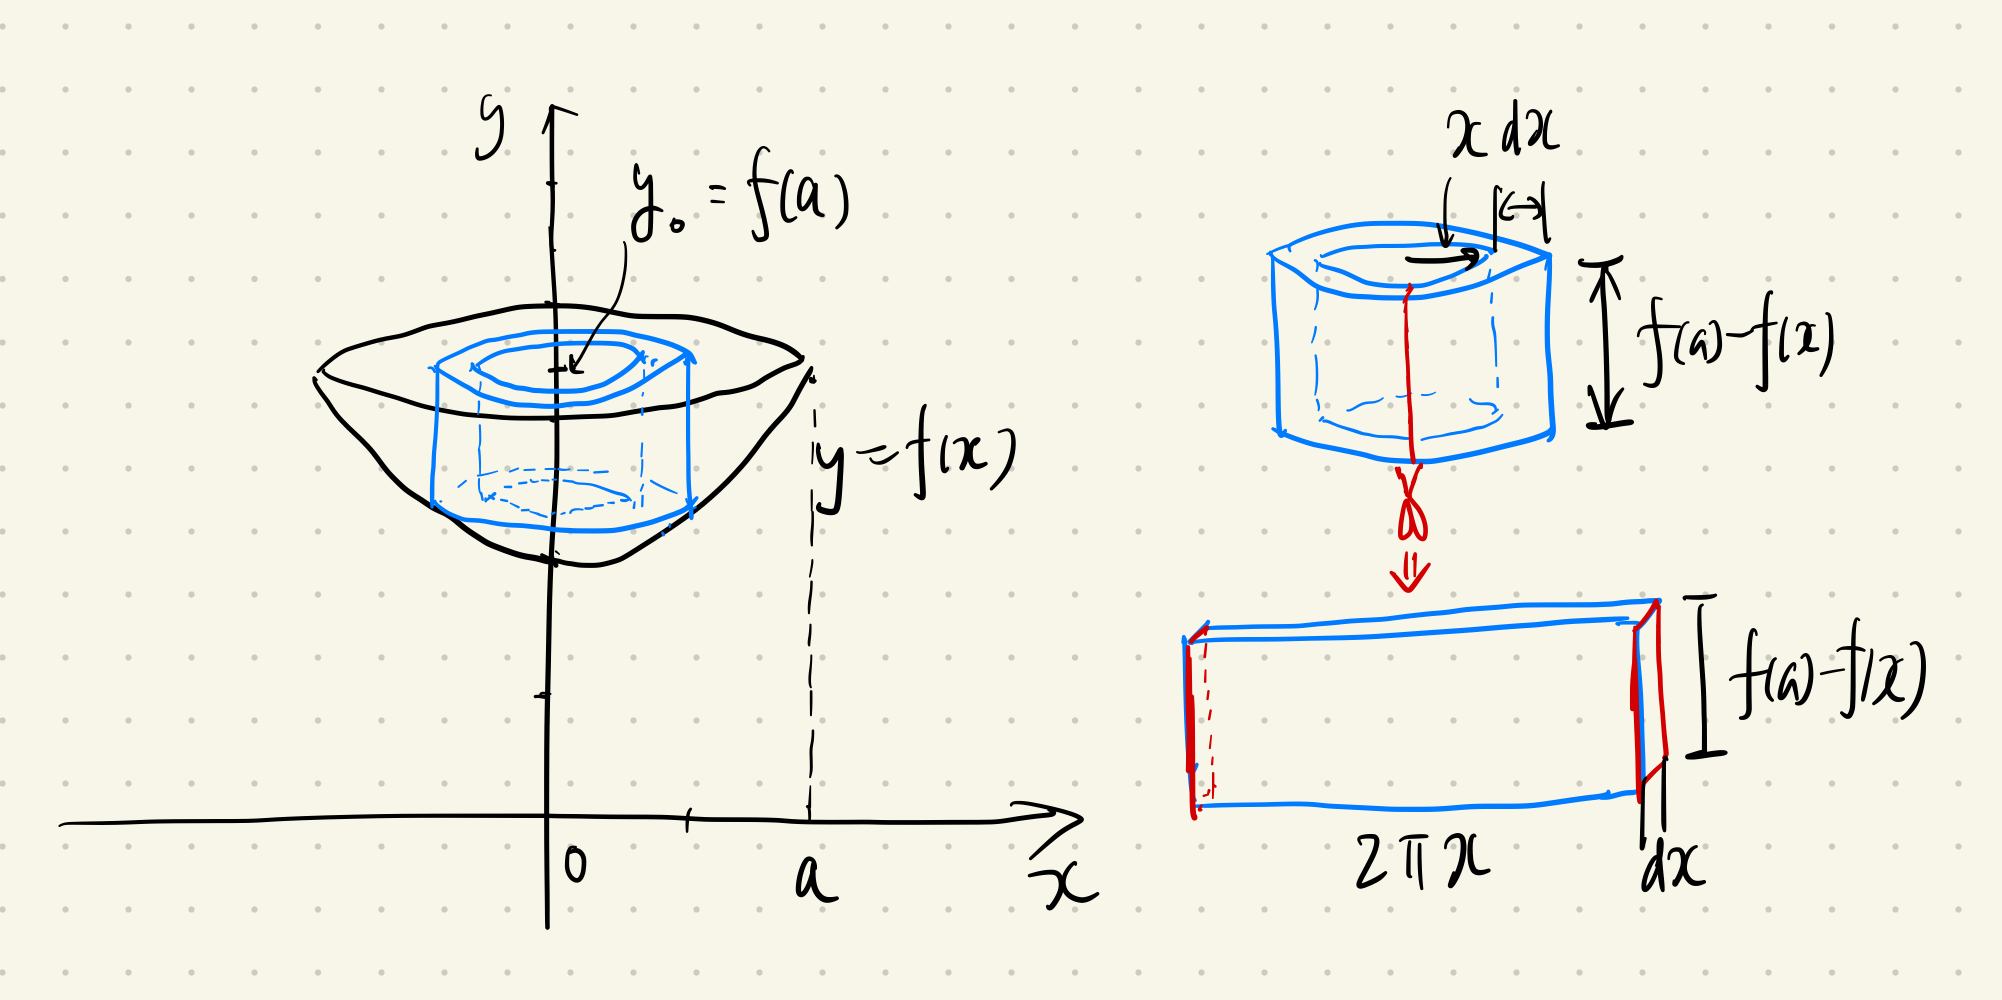
\includegraphics[width = 0.9\textwidth]{figures/chap 07/method_of_shells.png}
\end{figure}

\medskip
Aside from the method of disks, we still have another trick up our sleeves that can help us evaluate the volume of a solid of revolution.  Suppose we would like to find the volume of the solid constructed by revolving the area between the $y$-axis and $y = f(x)$ from $x = 0$ to $x = a$ around the $y$-axis.  In the method of disks, we would slice up the solid along the $y$-axis so that each slice is a thin disk.  However, we can alternatively slice up the solid into thin cylindrical shells with inner radius $x$ and thickness, as shown in the graph above.  The height of the shells depends on how the function behaves, but in this case it is $f(a)-f(x)$.  The solid can then be seen as a collection of thin shells with inner radius $x$ ranging from $0$ to $a$.  To derive the volume of each thin shell, we can cut it open as in the right panel and we would get a thin sheet with thickness $dx$, width $2 \pi x$ and height $f(a) - f(x)$.  Therefore, the volume of the thin shell is
\[2\pi x (f(a)-f(x))~dx\]
and the volume of the solid of revolution can be found by the integral
\[V = \int_0^a 2\pi x (f(a)-f(x))~dx\]
Since this method slices the solid of revolution into shells, it is terms as the \textit{method of shells}.  We now show how it works with the following example:

\begin{eg}[]{eg: rev_solid_vol_y_shell}
    Find the volume of the solid constructed by revolving the area between the $x$-axis and the curve of $y = e^x - x$ from $x = 0$ to $x = 1$ around the $y$-axis. 
\end{eg}

\begin{egsol}[]{exsol: rev_solid_vol_y_shell}
    \begin{center}
        \includegraphicsex{width = 0.7\textwidth, draft}{width = 0.7\textwidth}{figures/chap 07/method_of_shells_eg.png}
    \end{center}

    \medskip
    If we sketch out the solid, it is shaped like a cylinder with a bowl-like dent on the top, as shown in the graph above.  If we try to use the method of disks / rings to solve for it volume, then we will have to slice up the solid along the $y$-axis.  The bottom part of the slices will be easy to tackle, since they are all disks of radius $1$.  However, when we get to the top part with the dent, we will get rings instead of disks, and the inner radius of the rings will not be tractable since we will have to solve for $x$ in $y = e^x - x$. 
    
    Since the method of disks / rings is not viable for this problem, we turn to the method of shells.  If we slice the solid into concentric thin shells with inner radius $x$ and thickness $dx$, then the height of the shells, from the graph, would be $e^x - x$.  Therefore, the volume of the shells would be $2 \pi x (e^x-x)~dx$, and the volume of the solid can be obtained by integrating the volume of shells with $x$ going from $0$ to $1$:
    \begin{align*}
        \int_0^1 2 \pi x (e^x-x)~dx &= 2\pi\Big[\int_0^1 xe^x~dx - \int_0^1 x^2~dx\Big]\\
        &= 2\pi\Big[xe^x\big]_0^1 - \int_0^1 e^x~dx - \int_0^1 x^2~dx\Big]\\
        &= 2\pi\Big[xe^x\big]_0^1 - e^x\big]_0^1 - \frac{1}{3}x^3\big]_0^1\Big] = 2\pi\Big[e - (e - 1) - \frac{1}{3}\Big] = \frac{4}{3}\pi
    \end{align*}
\end{egsol}

We have now known how to evaluate the volume for a solid of revolution using definite integrals.  A natural follow-up question is that how do we find the surface area for a solid of revolution.  The approach we are taking is basically the same as finding arc lengths, only that now we are not chopping the curve into small segments, but slicing the surface area into "onion rings" demonstrated below, where we are trying to find the surface area for the solid revolving $y = f(x)$ from $x = a$ to $x = b$ around the $x$-axis:

\begin{figure}[ht]
    \centering
    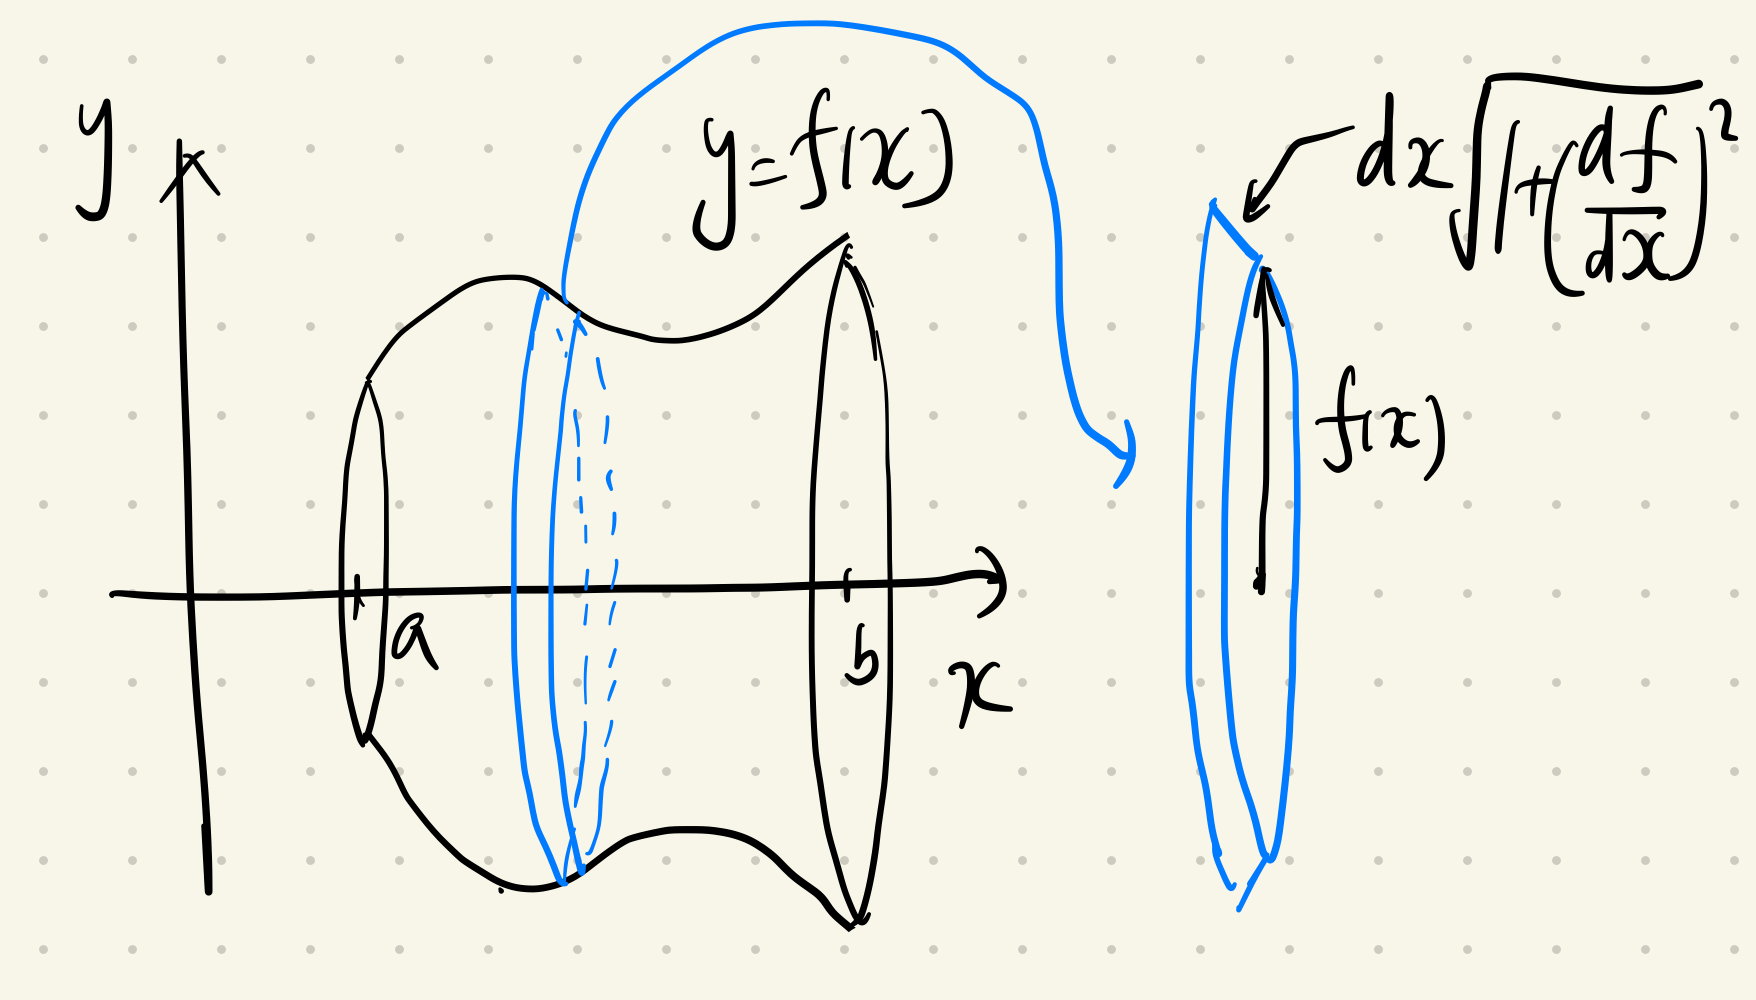
\includegraphics[width = 0.7\textwidth]{figures/chap 07/surface_area.png}
\end{figure}

here the slanted width of the ring is exactly the length of small segment in the derivation of arc lengths, so the width is also $\sqrt{1+(df(x)/dx)^2}~dx$.  Since this slanted width is revolved around the $x$-axis with radius $f(x)$ to form the surface of the solid, the surface area it sweeps through would be
\[2\pi f(x) \sqrt{1+\Big(\frac{df(x)}{dx}\Big)^2}~dx\]
Therefore, the surface area of the whole solid (excluding the left and right round caps by default) can be evaluated by integrating the surface area of the ring where $x$ goes from $a$ to $b$:
\[A = \int_a^b 2\pi f(x) \sqrt{1+\Big(\frac{df(x)}{dx}\Big)^2}~dx\]
We will end this section demonstrating how the surface area of balls and cones can also be evaluated using integrals.

\begin{eg}[]{eg: rev_solid_surf}
    Verify the surface area of the following solids
    \begin{enumerate}[a)]
        \item A ball of radius $r$ has surface area $4\pi r^2$.
        \item The lateral surface area of a cone of height $h$ and radius of base $r$ is $\pi r \sqrt{r^2+h^2}$.
    \end{enumerate}
\end{eg}

\begin{egsol}[]{egsol: rev_solid_surf}
    \begin{enumerate}[a)]
        \item As we have elaborate previously, a ball of radius $r$ can be constructed by revolving $y = f(x) = \sqrt{r^2-x^2}$ about the $x$-axis, as shown in the graph below. 
        \begin{center}
            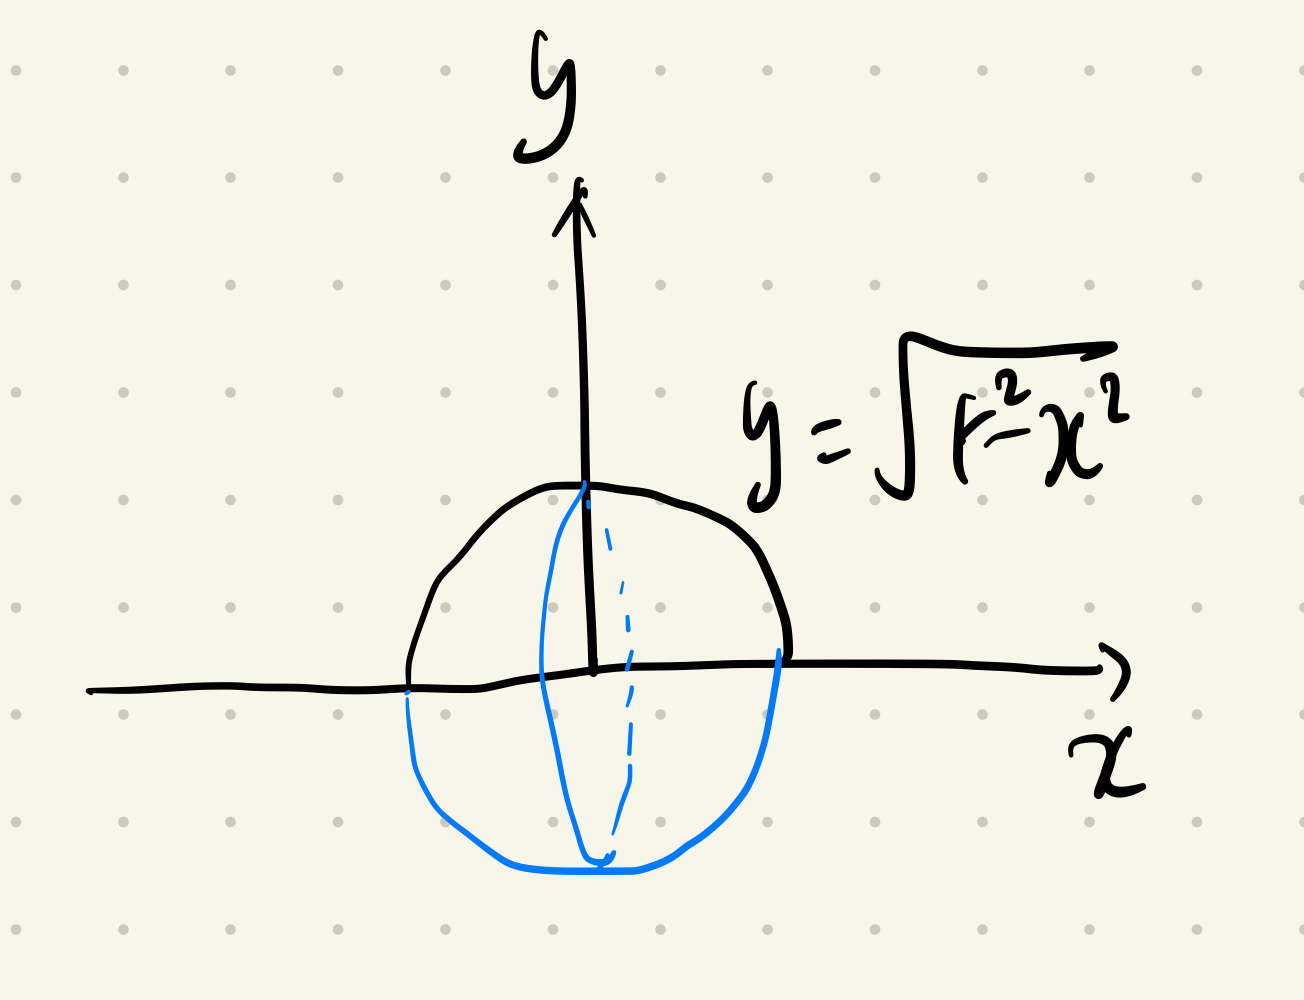
\includegraphics[width = 0.3\textwidth]{figures/chap 07/rev_solid_ball.png}
        \end{center}
        Therefore, we can use our formula to find the surface area of the ball:
        \begin{align*}
            A &= \int_{-r}^r 2 \pi f(x)\sqrt{1+\Big(\frac{df(x)}{dx}\Big)^2}~dx\\
            &= \int_{-r}^r 2 \pi \sqrt{r^2-x^2}\sqrt{1+\Big(\frac{-x}{\sqrt{r^2-x^2}}\Big)^2}~dx\\
            &= \int_{-r}^r 2 \pi \sqrt{r^2-x^2}\sqrt{\frac{r^2}{r^2-x^2}}~dx\\
            &= \int_{-r}^r 2 \pi r~dx = 2 \pi r x\big]_{-r}^r = 4 \pi r^2
        \end{align*}
        \item We have shown that if we revolve $y = f(x) = (r/h)x$ from $x = 0$ to $x = h$ around the $x$-axis, we would arrive at the cone for our problem, shown in the graph below:
        \begin{center}
            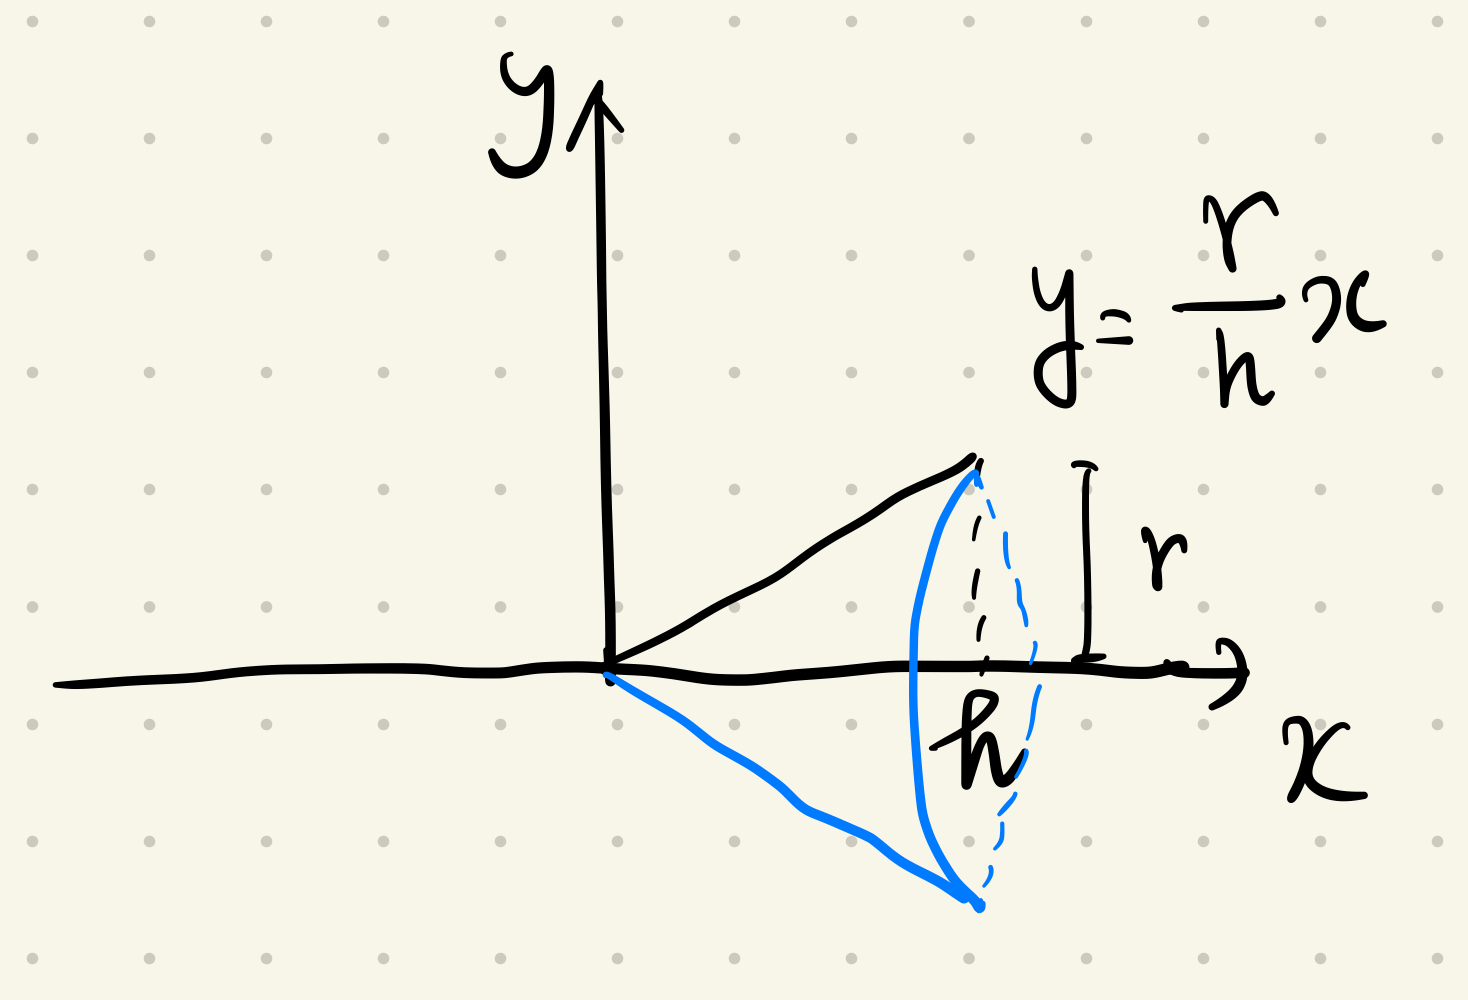
\includegraphics[width = 0.3\textwidth]{figures/chap 07/rev_solid_cone.png}
        \end{center}
        \allowdisplaybreaks
        Therefore, we can use our formula to find the lateral surface area of the cone:
        \begin{align*}
            A &= \int_0^h 2 \pi f(x)\sqrt{1+\Big(\frac{df(x)}{dx}\Big)^2}~dx\\
            &= \int_0^h 2 \pi \frac{r}{h} x \sqrt{1+\Big(\frac{r}{h}\Big)^2}~dx\\
            &= \int_0^h 2 \pi \frac{r\sqrt{r^2+h^2}}{h^2} x~dx = 2 \pi \frac{r\sqrt{r^2+h^2}}{h^2} \cdot \frac{1}{2}x^2\Big]_0^h = 2 \pi \frac{r\sqrt{r^2+h^2}}{h^2} \cdot \frac{1}{2}h^2 = \pi r \sqrt{r^2+h^2}
        \end{align*}
    \end{enumerate}
\end{egsol}

\section{Improper integrals}
Up until now, when we are talking about definite integrals shaped as the following:
\[\int_a^b f(x) dx\]
we require (1) $a$ and $b$ are real numbers and cannot be $\pm \infty$ (2) $f(x)$ is continuous within $[a,b]$.  However, in certain applications, we would want to relax these requirements.  For example, we may want to evaluate the area under curve for $y = e^{-x}$ over the whole positive real line, then we would use the expression
\[\int_0^\infty e^{-x}~dx\]
where the upper limit of integration is $\infty$.  Or, we would want to know the area under curve for $y = \frac{1}{|\sqrt[3]{x}|}$ between $x = -1$ and $x = 1$, then we would need the evaluate
\[\int_{-1}^1 \frac{1}{|\sqrt[3]{x}|}~dx\]
However, $\frac{1}{|\sqrt[3]{x}|}$ tends to positive infinity when $x$ approaches $0$ from either side, so it has an infinite discontinuity at $x=0$.  These types of definite integrals are called \textbf{improper integrals}, and can be given a concrete definition using limits.  We first deal with the case where the limits of integration goes to $\pm \infty$:

\begin{defi}[Improper integrals with infinite limits of integration]{def: improper_inf}
    \begin{enumerate}
        \item If $f(x)$ is continuous within $[a, \infty)$, then
        \[\int_a^{\infty} f(x)dx = \lim_{b \rightarrow \infty} \int_a^b f(x)dx\]
        \item If $f(x)$ is continuous within $(-\infty, b]$, then
        \[\int_{-\infty}^b f(x)dx = \lim_{a \rightarrow -\infty} \int_a^b f(x)dx\]
        \item If $f(x)$ is continuous within $\mathbb{R}$, then
        \[\int_{-\infty}^{\infty} f(x)dx = \int_{-\infty}^c f(x)dx + \int_c^{\infty} f(x)dx\]
        where $c$ is any real number.
    \end{enumerate}
\end{defi}

This implies that when evaluating improper integrals with $\pm \infty$ at either limit of integration, after the phase of finding the antiderivative, we can interpret the step of "evaluating the antiderivative at $\pm 
\infty$" as taking the limit of the antiderivative as the variable of interest goes to $\pm \infty$.  Also note that in the definition above, if any of the limit on the right hand side does not exist, then we say that the improper integral to be evaluated does not exist or \textit{diverges}.

\begin{eg}[]{eg: improper_inf}
    Evaluate the following improper integrals:
    \begin{tasks}(3)
        \task $\int_0^\infty e^{-x}~dx$
        \task $\int_0^\infty \frac{1}{x^2+1}~dx$
        \task $\int_0^\infty xe^{-x}~dx$
        \task $\int_{-\infty}^1 \sqrt{3-x}~dx$
        \task $\int_{-\infty}^{-1} \frac{e^{1/x}}{x^2}~dx$
        \task $\int_{-\infty}^{\infty} \frac{x^3}{(x^4+1)^2}~dx$
    \end{tasks}
\end{eg}

\begin{egsol}[]{egsol: improper_inf}
    \begin{enumerate}[a)]
        \item Since there is an infinity in the upper limit of integration, we may transform this improper integral into a limit by definition:
        \begin{align*}
            \int_0^\infty e^{-x} dx &= \lim_{b \rightarrow \infty} \Big[\int_0^b e^{-x} dx\Big]\\
            &= \lim_{b \rightarrow \infty} \Big[-e^{-x}\big]_0^b \Big]\\
            &= \lim_{b \rightarrow \infty} \Big[(-e^{-b}) - (-e^{0})\Big]\\
            &= \big[\lim_{b \rightarrow \infty} (-e^{-b})\big] + 1 = 1
        \end{align*}
        Alternatively, we can avoid writing a lot of limit signs and treat the $\infty$ symbol as sort of a number (although it isn't!), and remember that evaluating any expression at $\infty$ is actually taking the limit of that expression at $\infty$:
        \[\int_0^\infty e^{-x} dx = -e^{-x}\Big]_0^\infty = \big[\lim_{x \rightarrow \infty} (-e^{-x})\big] - (- e^0) = 1\]
        \item Here the upper limit is $\infty$, so the integral is an improper integral, and we should evaluate the integral with limits:
        \[\int_0^\infty \frac{1}{x^2+1}~dx = \arctan x\Big]_0^\infty = \big[\lim_{x \rightarrow \infty} \arctan x\big] - \arctan 0 = \frac{\pi}{2} - 0 = \frac{\pi}{2}\]
        Here $\lim_{x \rightarrow \infty} \arctan x = \pi/2$ since as $\theta$ approaches $\pi/2$ from the left side, $\tan \theta$ shoots up to $\infty$.
        \item The shape of this integrand hints us to use integration by parts, setting $u = x$, $dv/dx = e^{-x}$ so that $du/dx = 1$, $v = -e^{-x}$.  Note that since this is an improper integral with infinite integration limits, the "$uv$" term in the integration by parts will also need to be evaluated with limits:
        \begin{align*}
            \int_0^\infty xe^{-x}~dx &= x(-e^{-x})\Big]_0^\infty - \int_0^\infty 1\cdot(-e^{-x})~dx\\
            &= x(-e^{-x})\Big]_0^\infty - e^{-x}\Big]_0^\infty\\
            &= \Big[\big[\lim_{x \rightarrow \infty} (-xe^{-x})\big] - 0)\Big] - \Big[\lim_{x \rightarrow \infty} e^{-x} - 1\Big]
        \end{align*}
        For the first limit, we can use L'Hôpital's rule since if we write $-xe^{-x}$ as $\frac{-x}{e^x}$, we get an $\frac{-\infty}{\infty}$ indefinite form from the plug-in method:
        \[\lim_{x \rightarrow \infty} -xe^{-x} = \lim_{x \rightarrow \infty} \frac{-x}{e^x} = \lim_{x \rightarrow \infty} \frac{(-x)'}{(e^x)'} = \lim_{x \rightarrow \infty} \frac{-1}{e^x} = \lim_{x \rightarrow \infty} -e^{-x} = 0\]
        Therefore, our integral evaluates to 
        \[\Big[\big[\lim_{x \rightarrow \infty} (-xe^{-x})\big] - 0)\Big] - \Big[\lim_{x \rightarrow \infty} e^{-x} - 1\Big] = \Big[0 - 0\Big] - \Big[0 - 1\Big] = 1\]
        \item For this integrand, clearly we need to do a U-substitution with $u = 3-x$, so that $du = -dx$.  Since this is a (improper) definite integral, we have to substitute the limits of integration as well: when $x = 1$, we have $u = 3 - 1 = 2$; when $x$ goes to $-\infty$, then $u$ goes to $\infty$.  Therefore we have
        \begin{align*}
            \int_{-\infty}^1 \sqrt{3-x}~dx &= - \int_{-\infty}^1 \sqrt{3-x}~(-dx)\\
            &= - \int_{\infty}^2 \sqrt{u}~du\\
            &= \int_2^{\infty} u^{1/2}~du\\
            &= \frac{2}{3}u^{3/2}\Big]_2^{\infty}\\
            &= \lim_{u \rightarrow \infty} \frac{2}{3}u^{3/2} - \frac{2}{3} 2^{3/2}
        \end{align*}
        Since the first limit term goes to $\infty$, the whole improper integral goes to $\infty$.  So we have
        \[\int_{-\infty}^1 \sqrt{3-x}~dx = \infty\]
        \item For this integrand, we can do a U-substitution for the exponent so that $u = \frac{1}{x}$ and $du = -\frac{1}{x^2} dx$, which yields a multiple of the remainder of the integrand, $\frac{1}{x^2}$.  We will also need to substitute the limits of integration: when $x = -1$, we have $u = \frac{1}{-1} = -1$; when $x$ goes to $-\infty$, then $u$ goes to $0$ from the negative side.  Therefore we have,
        \[\int_{-\infty}^{-1} \frac{e^{1/x}}{x^2}~dx = -\int_{-\infty}^{-1} e^{1/x}\Big(-\frac{1}{x^2}~dx\Big) = -\int_{0}^{-1} e^u~du = \int_{-1}^0 e^u~du = e^u\Big]_{-1}^0 = 1 - e^{-1}\]
        \item For this integrand, we can try U-substitution for the expression within the parentheses.  This yields $u = x^4+1$ and $du = 4x^3~dx$, which works since $x^3$ appears in the integrand as the remainder.  We will also need to substitute the limits of integreation: when $x$ goes to $\infty$, $u$ also goes to $\infty$; when $x$ goes to $-\infty$, $u$ also goes to $\infty$.  Therefore,
        \[\int_{-\infty}^{\infty} \frac{x^3}{(x^4+1)^2}~dx = \frac{1}{4}\int_{-\infty}^{\infty} \frac{1}{(x^4+1)^2}~(4x^3dx) = \frac{1}{4}\int_{\infty}^{\infty}\frac{1}{u^2}~du = -\frac{1}{4u}\Big]_{\infty}^{\infty} = 0 - 0 = 0\]
        This integral eventually evaluates to $0$ since the integrand $f(x) := \frac{x^3}{(x^4+1)^2}$ is an \textit{odd function}, which means that $f(x) = -f(-x)$ for all $x$.  Therefore, when we graph the integrand on the Cartesian plane, the curve at the left side of the plane is just flipping the curve on the right side of the plane about the $y$-axis then the $x$-axis, as shown in the graph below: 
        \begin{center}
            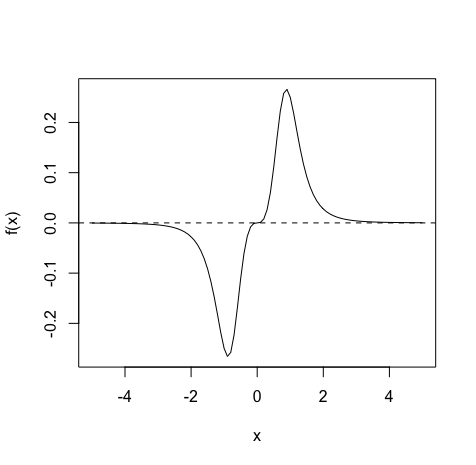
\includegraphics[trim = {0 0 0 2cm}, clip, width = 0.6\textwidth]{figures/chap 07/odd_function.png}
        \end{center}
        Therefore, when we integrate over the whole real line, the negative signed area on the left side of the plane cancels out the with positive signed area on the right, leading to an integral of zero.  (A subtlty here is that, even if the integrand is an odd function, the area under curve on the right side of the plane must be finite for us to conclude that the whole improper integral evaluates to $0$.  Otherwise, we would get an $\infty - \infty$ indeterminate form and the improper integral just does not exist.  You may try evaluating $\int_{-\infty}^{\infty} x~dx$ to see this.)
    \end{enumerate}
\end{egsol}

There is still one case that makes a definite integral improper, which is when the integrand has one or several infinite discontinuities within the limits or integration.  We now provide a definition for how this type of improper integral should be evaluated:

\pagebreak

\begin{defi}[Improper integrals with infinite discontinuities]{def: improper_dis}
    \begin{enumerate}
        \item If $f(x)$ is continuous within $[a, b)$ and has an infinite discontinuity at $x = b$, then
        \[\int_a^b f(x)dx = \lim_{c \rightarrow b^-} \int_a^c f(x)dx\]
        \item If $f(x)$ is continuous within $(a, b]$ and has an infinite discontinuity at $x = a$, then
        \[\int_a^b f(x)dx = \lim_{c \rightarrow a^+} \int_c^b f(x)dx\]
        \item If $f(x)$ is continuous within $[a, b]$ except for $x = c \in [a, b]$, where it has an infinite discontinuity, then
        \[\int_a^b f(x)dx = \int_a^c f(x)dx + \int_c^b f(x)dx\]
    \end{enumerate}
\end{defi}

The first two definitions imply that when the infinite discontinuities occur at the limits of integration, we can proceed with normal procedures for definite integrals, and take limits when plugging values into the antiderivatives as needed.  The third definition presents a pitfall: if $F(x)$ is one of the antiderivative for $f(x)$, then we should evaluate the integral by
\[\big[\lim_{t \rightarrow c^-} F(t)\big] - F(a) + F(b) - \big[\lim_{t \rightarrow c^+} F(t)\big]\]
When either of the two limits does not exist, then the improper integral diverges.  However, if we erroneously ignored the infinite discontinuity and just evaluated $F(b)-F(a)$ as we often do in proper integrals, we will not be able to realize that the improper integral actually diverges. 

Let us see how this type of improper integrals should be evaluated in the examples below:

\begin{eg}[]{eg: improper_dis}
    Evaluate the following improper integrals:
    \begin{tasks}(3)
        \task $\int_0^1 \frac{1}{\sqrt[3]{x}}~dx$
        \task $\int_0^1 \frac{1}{x^3}~dx$
        \task $\int_{0}^{\infty} \frac{1}{\sqrt{x}(x+1)}~dx$
        \task $\int_{-2}^1 \frac{1}{x^2}~dx$
        \task $\int_1^3 \frac{x}{x^2-4}~dx$
        \task $\int_1^6 \frac{x}{\sqrt[3]{x^2-9}}~dx$
    \end{tasks}
\end{eg}

\begin{egsol}[]{egsol: improper_dis}
    \begin{enumerate}[a)]
        \allowdisplaybreaks
        \item The integrand has an infinite discontinuity at the lower limit of integration $x = 0$.  Therefore, we can rewrite the lower limit as $0^+$ to remind us to take the limit after finding the antiderivative and proceed on: 
        \[\int_0^1 \frac{1}{\sqrt[3]{x}}~dx = \int_{0^+}^1 x^{-1/3}~dx = \frac{3}{2}x^{2/3}\Big]_{0^+}^1 = \frac{3}{2} - 0 = \frac{3}{2}\]
        Note that since $x^{2/3}$ is actually continuous at $x = 0$, so we can just plug $0$ into $x$ and obtain the right limit.
        \item The integrand has an infinite discontinuity at the lower limit of integration $x = 0$.  We use the same approach and write $0$ as $0^+$:
        \[\int_0^1 \frac{1}{x^3}~dx = \int_{0^+}^1 x^{-3}~dx = -\frac{1}{2}x^{-2}\Big]_{0^+}^1 = -\frac{1}{2} - \lim_{x \rightarrow 0^+} \Big(-\frac{1}{2x^2}\Big) = \infty\]
        Here as $x$ approaches $0$ from the right side, the limit approaches negative infinity since the denominator is a positive number that gets smaller and smaller.  Therefore, the whole expression goes to positive infinity since there is a negative sign before the limit.
        \item Here we have two elements that makes this integral improper: we have an infinite upper limit for integration, as well as an infinite discontinuity at $x = 0$, which is the lower limit for integration.  We therefore write the lower limit as $0^+$ and proceed on finding the antiderivative for the integrand, which can be done by first noting we can write integrand as 
        \[\frac{1}{\sqrt{x}(x+1)} = \frac{1}{\sqrt{x}((\sqrt{x})^2+1)}\]
        Therefore, we can use U-substitution with $u = \sqrt{x}$, $du = \frac{1}{2\sqrt{x}}dx$.  For the integration limits, as $x$ goes to $\infty$, $u$ also goes to $\infty$; as $x$ approaches $0$ from the right side, $u$ also approaches $0$ from the right side.  Now we have
        \begin{align*}
            \int_0^{\infty} \frac{1}{\sqrt{x}(x+1)}~dx &= \int_{0^+}^{\infty} \frac{1}{\sqrt{x}(x+1)}~dx\\
            &= 2\int_{0^+}^{\infty} \frac{1}{(\sqrt{x})^2+1}~\Big(\frac{1}{2\sqrt{x}}dx\Big)\\
            &= 2\int_{0^+}^{\infty} \frac{1}{u^2+1}~du\\
            &= 2 \arctan u\Big]_{0^+}^{\infty} = 2\Big(\frac{\pi}{2} - 0\Big) = \pi
        \end{align*}
        In the last line, we have shown in the previous example that $\arctan x$ goes to $\pi/2$ as $x$ goes to $\infty$.  Also, since $\arctan x$ is continuous at $x = 0$, its right limit at $x = 0$ can be found with the plugin method, leading to $\arctan 0 = 0$. 
        \item In this integral, since the integrand $1/x^2$ has an infinite discontinuity at $x = 0$, we have to split up the integral into integrating from $-2$ to $0$ and from $0$ to $1$:
        \[\int_{-1}^2 \frac{1}{x^2}~dx = \int_{-1}^{0} \frac{1}{x^2}~dx + \int_{0}^2 \frac{1}{x^2}~dx\]
        Now the two new integrals have infinite discontinuties at their upper or lower integration, so we write $0$ as $0^-$ and $0^+$, then proceed on to antidifferentiation:
        \begin{align*}
            \int_{-1}^{0} \frac{1}{x^2}~dx + \int_{0}^2 \frac{1}{x^2}~dx &= \int_{-1}^{0^-} \frac{1}{x^2}~dx + \int_{0^+}^2 \frac{1}{x^2}~dx\\
            &= \big(-\frac{1}{x}\big)\Big]_{-1}^{0^-} + \big(-\frac{1}{x}\big)\Big]_{0^+}^{2}\\
            &= \Big[\lim_{x \rightarrow 0^-} \big(-\frac{1}{x}\big) - 1\Big] + \Big[-\frac{1}{2}-\lim_{x \rightarrow 0^+} \big(-\frac{1}{x}\big)\Big]
        \end{align*}
        Now since the first limit goes to positive infinity and the second limit goes to negative infinity, the improper integral goes to \textbf{positive infinity}.  Note that if we carelessly ignored the infinite discontinuity, we would get 
        \[\int_{-1}^2 \frac{1}{x^2}~dx = -\frac{1}{x}\Big]_{-1}^2 = \big(-\frac{1}{2}\big)-1 = -\frac{3}{2}\]
        which is clearly incorrect (note that the integrand $1/x^2$ is always positive).
        \item For this integral, we have an infinite discontinuity for the integrand at $x = 2$, so we have to split the integral as
        \[\int_1^3 \frac{x}{x^2-4}~dx = \int_1^{2^-} \frac{x}{x^2-4}~dx + \int_{2^+}^3 \frac{x}{x^2-4}~dx\]
        where we write $2$ as $2^-$ and $2^+$ to remind us to take the left and right limits when evaluating the antiderivatives.  Now the integrand can be antidifferentiated with U-substitution where $u = x^2-4$ and $du = 2xdx$.  For the integration limits, when $x = 1$ we have $u = -3$, when $x = 3$ we have $u = 5$, when $x$ approaches $2$ from the left and right side we have $u$ approaching $0$ from the left and right side.  Therefore,
        \begin{align*}
            \int_1^{2^-} \frac{x}{x^2-4}~dx + \int_{2^+}^3 \frac{x}{x^2-4}~dx &= \frac{1}{2}\int_1^{2^-} \frac{1}{x^2-4}~(2xdx) + \frac{1}{2} \int_{2^+}^3 \frac{1}{x^2-4}~(2xdx)\\
            &= \frac{1}{2}\int_{-3}^{0^-} \frac{1}{u}du + \frac{1}{2}\int_{0^+}^5 \frac{1}{u}du\\
            &= \frac{1}{2} \ln|u|\big]_{-3}^{0^-} + \frac{1}{2} \ln|u|\big]_{0^+}^{5}\\
            &= \frac{1}{2}\Big[\lim_{u \rightarrow 0^-} \ln|u| - \ln 3\Big] + \frac{1}{2}\Big[\ln 5-\lim_{u \rightarrow 0^+} \ln|u|\Big]
        \end{align*}
        Now both limits in the last line evaluate to $-\infty$, so the expression becomes a $\infty - \infty$ indeterminate form.  Therefore, this improper integral simply \textbf{does not exist}.  Note that if we ignored the infinite discontinuity, we would get a wrong answer of $\frac{1}{2}\ln\frac{5}{3}$. 
        \item In this integral, we have an infinite discontinuity for the integrand at $x = 3$, so we have to split the integral as
        \[\int_1^6 \frac{x}{\sqrt[3]{x^2-9}}~dx = \int_1^{3^-} \frac{x}{\sqrt[3]{x^2-9}}~dx + \int_{3^+}^6 \frac{x}{\sqrt[3]{x^2-9}}~dx\]
        where we again write $3$ as $3^-$ and $3^+$.  The integrand can be antidifferentiated with U-substitutioin setting $u = x^2-9$ and $du = 2dx$.  For the integration limits, when $x = 1$ we have $u = -8$, when $x = 6$ we have $u = 27$, and when $x$ approaches $3$ from the left and right side we have $u$ approaching $0$ from the left and right side.  Therefore,
        \begin{align*}
            \int_1^{3^-} \frac{x}{\sqrt[3]{x^2-9}}~dx + \int_{3^+}^6 \frac{x}{\sqrt[3]{x^2-9}}~dx &= \frac{1}{2}\int_1^{3^-} \frac{1}{\sqrt[3]{x^2-9}}~(2xdx) + \frac{1}{2}\int_{3^+}^6 \frac{1}{\sqrt[3]{x^2-9}}~(2xdx)\\
            &= \frac{1}{2}\int_{-8}^{0^-} \frac{1}{\sqrt[3]{u}}~du + \frac{1}{2}\int_{0^+}^{27} \frac{1}{\sqrt[3]{u}}~du\\
            &= \frac{1}{2}\int_{-8}^{0^-} u^{-1/3}~du + \frac{1}{2}\int_{0^+}^{27} u^{-1/3}~du\\
            &= \frac{1}{2}\cdot\frac{3}{2} u^{2/3}\big]_{-8}^{0^-} + \frac{1}{2}\cdot\frac{3}{2} u^{2/3}\big]_{0^+}^{27}\\
            &= \frac{3}{4}[(\sqrt[3]{0})^2-(\sqrt[3]{-8})^2] + \frac{3}{4}[(\sqrt[3]{27})^2-(\sqrt[3]{0})^2]\\
            &= \frac{3}{4}(9-4) = \frac{15}{4}
        \end{align*}
        In the phase of antiderivative evaluation, since $u^{2/3}$ is continutous at $u=0$, we plug in $0$ to obtain the right and left limits (though they are eventually cancelled out). 
    \end{enumerate}
\end{egsol}

\section{Probability, expectation value and variance}
Integrals are also useful in statistics, which is a specialty that uses mathematical tools to extract information from data, and then produce predictions or draw conclusions based on the information.  The information within the data cannot be readily identified before the noise in the data is properly modelled and controlled.  Therefore, the tools statistician use relies heavily on probability, which can involve a bit of integrals.

Suppose we are interested in a quantity whose possible value ranges over a continuous interval of number, eg. the length of time customers spent waiting in a queue, the height of students within an univeristy, or the price of a stock over time.  Each time we observed this quantity, its value can vary randomly (eg. different students will have different heights).  Therefore, statisticians call these quantities \textbf{random variables}.  In particular, since the possible values for these random variables are continuous (unlike, say, the outcome of die, which can be only one of $1,2,3,4,5,6$), they are called \textbf{continuous random variables}. 

The most intuitive way to describe a random variable is to specify the probability of observing each possible value.  For example, for a fair die, we can describe the random variable for its outcome, denote as $X$, by
\[\PP(X=1) = \PP(X=2) = \PP(X=3) = \PP(X=4) = \PP(X=5) = \PP(X=6) = \frac{1}{6}\]
However, we cannot describe a continuous random variable as above, since the probability of observing each possible outcome is actually $0$ (eg. the probability of observing a student of exactly $168.523$ cm is $0$).  Therefore, for a continuous random variable $X$, we would describe it by providing its \textbf{probability density function} $f_X(x)$, so that
\[\PP(a \le X \le b) = \int_a^b f_X(x)~dx\]
That is, if we graph $f_X(x)$ on a Cartesian plane, then the area under curve for $f_X(x)$ between $x=a$ and $x=b$ is the probability of $X$ being between $a$ and $b$.  Under this definition, we will have two implications:
\begin{enumerate}
    \item Since the area under curve for $f_X(x)$ represents probability, $f_X(x)$ cannot be negative or we will sometimes derive negative probabilities.
    \item Since $X$ will always be between $-\infty$ to $\infty$, the probability of "$-\infty \le X \le \infty$ would be $1$.
\end{enumerate}
We can write these two requirements for probability density functions as follows:
\begin{gather*}
    f_X(x) \ge 0, \text{ for all }x\\
    \int_{-\infty}^{\infty} f_X(x)~dx = 1
\end{gather*}
Let's look at how probability density functions work with the following example:
\begin{eg}[]{eg: pdf}
    Suppose the random variable for the waiting time (in minutes) for a queue of customers is denoted as $X$.  The probability density function for $X$ is 
    \[f_X(x) = \begin{cases}
        \frac{1}{2}e^{-\frac{x}{2}}, x \ge 0\\
        0, \quad \;\; x < 0
    \end{cases}\]
    \begin{enumerate}[a)]
        \item Verify that $f_X(x)$ is a probability density function.
        \item Calculate the probability of a customer waiting between $1$ to $2$ minutes.
        \item Calculate the probability of a customer waiting less than $1$ minute.
    \end{enumerate}
\end{eg}

\begin{egsol}[]{egsol: pdf}
    \begin{enumerate}[a)]
        \item The two requirements for a function to be a probability density function is that (1) it is non-negative for all inputs (2) its area under curve over the real line, i.e. definite integral from $-\infty$ to $\infty$, is $1$.  The first requirement is trivial since the exponential function is always non-negative.  For the second requirement, since $f_X(x)$ is defined piecewisely, we can also seperate the integral into two parts
        \[\int_{-\infty}^{\infty} f_X(x)~dx = \int_{-\infty}^{0} f_X(x)~dx + \int_{0}^{\infty} f_X(x)~dx\]
        We can then plug in the expression for $f_X(x)$ in the respective range of integration and yield
        \begin{align*}
            \int_{-\infty}^{0} f_X(x)~dx + \int_{0}^{\infty} f_X(x)~dx &= \int_{-\infty}^{0} 0~dx + \int_{0}^{\infty} \frac{1}{2}e^{-\frac{x}{2}}~dx\\
            &= 0 + \big(-e^{-\frac{x}{2}}\big)\Big]_0^{\infty} = 0 - (-1) = 1
        \end{align*}
        which proves that $f_X(x)$ is a legit probabiltiy density function.
        \item The probabiltiy of a customer waiting between $1$ to $2$ minutes is exactly the probability of $1 \le X \le 2$, so we can write:
        \[\PP(1 \le X \le 2) = \int_1^2 f_X(x)~dx = \int_1^2 \frac{1}{2}e^{-\frac{x}{2}} = -e^{-\frac{x}{2}}\Big]_1^2 = e^{-\frac{1}{2}} - e^{-1}\]
        \item Since the waiting time cannot be negative (which is also implied by $f_X(x)$ begin zero when $x$ is negative), the probability of a customer waiting under $1$ minute is the probability of $0 \le X \le 1$, so we can write:
        \[\PP(0 \le X \le 1) = \int_0^1 f_X(x)~dx = \int_0^1 \frac{1}{2}e^{-\frac{x}{2}}~dx = -e^{-\frac{x}{2}}\Big]_0^1 = 1-e^{-\frac{1}{2}}\]
    \end{enumerate}
\end{egsol}

With the probability density function in hand, we can then calculate the two most important charateristics of a (continuous) random variable: its \textbf{expected value} and \textbf{variance}.  A random variable's expected value is the average value that you would see from this random variable.  For example, suppose $X$ represents the waiting time of customers in the queue, then the expected value for $X$, often written as $\EE[X]$, is the average time of waiting.  To gauge how to derive the expected value using probability density functions, let us first go back to the die example again.  When a fair die is rolled, the expected value for its outcome $X$ is intuitively
\[\EE[X] = \frac{1+2+3+4+5+6}{6} = 3.5\] 
which is just the average of all outcomes.  Alternatively, we can write the above equation as
\[\EE[X] = 1 \cdot \frac{1}{6} + 2 \cdot \frac{1}{6} + 3 \cdot \frac{1}{6} + 4 \cdot \frac{1}{6} + 5 \cdot \frac{1}{6} + 6 \cdot \frac{1}{6} = 3.5\]
That is, we are multiplying the value of possible outcomes and their probabilities (which is uniformly $1/6$ for a fair die), and then summing all these products together.  If the die is not a fair die, and it always shows $4$, $5$, or $6$ with probability $\frac{1}{4}$, $\frac{1}{4}$ and $\frac{1}{2}$, then the expected value of its outcome would then be
\[\EE[X] = 4 \cdot \frac{1}{4} + 5 \cdot \frac{1}{4} + 6 \cdot \frac{1}{2} = 5.25\]

Now we're prepped for deriving the expected value of a continuous random variable.  Suppose a continuous random variable $X$ has probability denstiy function $f_X(x)$ graphed below.  Then, we can slice the $x$-axis into small strips, each strip representing a small range of possible values for $X$.  For the strip shown in the graph ranging from $x$ to $x+dx$, the probability of $x \le X \le x+dx$ would be the area under curve between $x$ and $x+dx$, which is approximately a rectangle of height $f_X(x)$ and width $dx$.  In the virtue of how we calculated the expected value of a die, we should multiply this probability with the outcome tied to it, which is $x$ to $x + dx$ and can basically be replaced by $x$, as $dx$ is small.  Therefore, the product contributed by this strip would be $x f_X(x) dx$, and eventually we want to add up the products provided by all strips to arrive at the expected value, which yields
\[\EE[X] = \int_{-\infty}^{\infty} x f_X(x)~dx\]

\begin{figure}[ht]
    \centering
    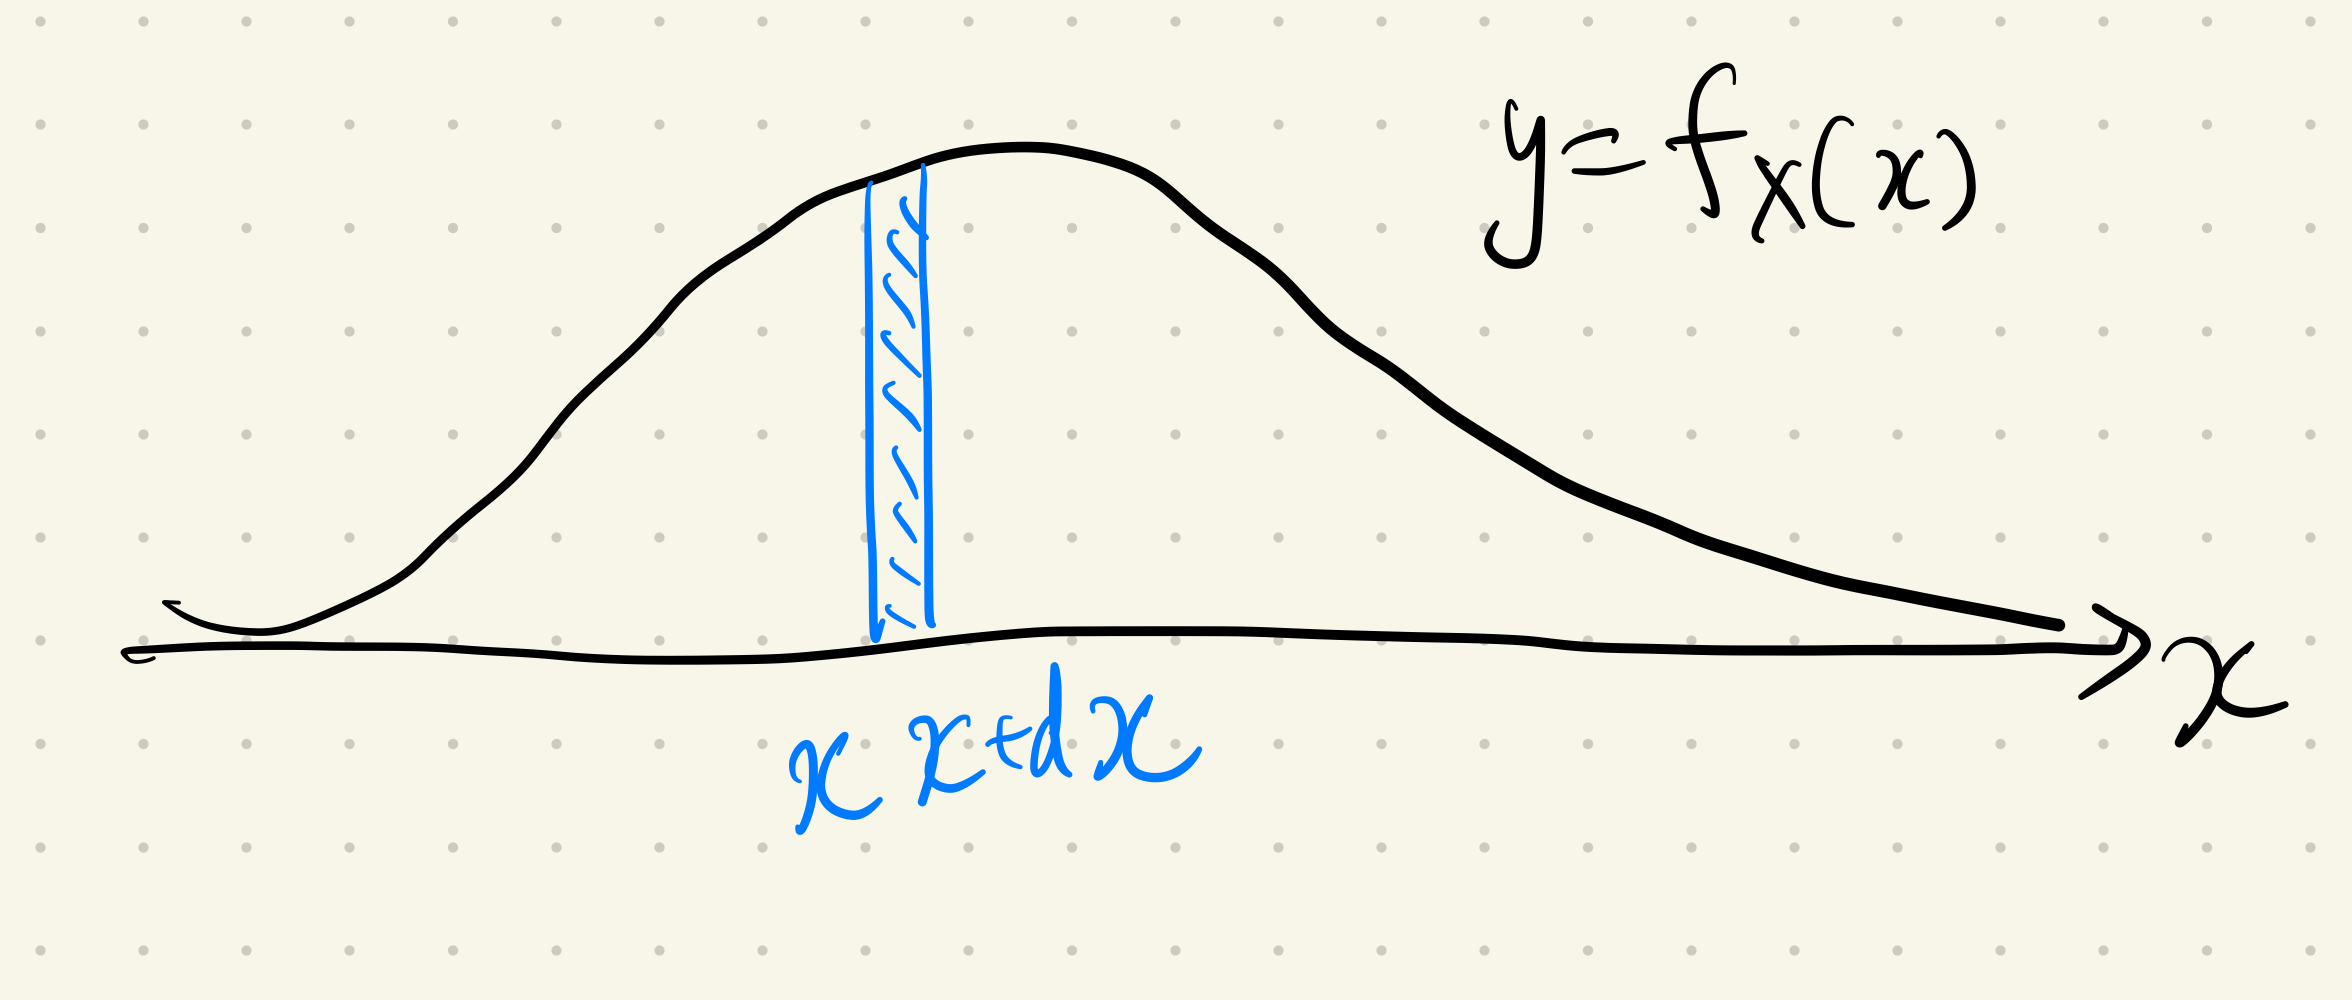
\includegraphics[width = 0.5\textwidth]{figures/chap 07/expectation.png}
\end{figure}

Another characteristic that is important to a random variable is its variance.  The variance is trying to measure how dispersed is the outcome of a random variable $X$ relative to its expectation value $\EE[X]$.  An intuitive way to define this dispersion is to find the expected value of the distance between $X$ and $\EE[X]$, which can be written as $\EE[|X - \EE[X]|]$.  However, this expression does not have good mathematical properties and is difficult to maneuver, so statistician prefer using the expected value of the squared distance between $X$ and $\EE[X]$.  Therefore, we have the definition of variance $var[X]$:
\[var[X] = \EE[(X-\EE(X))^2] = \int_{-\infty}^{\infty} (x - \EE[X])^2 f_X(x)~dx\]
In addition, we can expand the term $(x-\EE[x])^2$ in the integrand and arrive at another expression for the variance:

\pagebreak

\begin{align*}
    var[X] &= \int_{-\infty}^{\infty} (x-\EE[X])^2 f_X(x)~dx\\
    &= \int_{-\infty}^{\infty} (x^2 - 2x\EE[X] + (\EE[X])^2) f_X(x)~dx\\
    &= \int_{-\infty}^{\infty} x^2 f_X(x)~dx - 2\EE[X] \int_{-\infty}^{\infty} x f_X(x)~dx + (\EE[X])^2 \int_{-\infty}^{\infty} f_X(x)~dx\\
    &= \EE[X^2] - 2 \EE[X] \EE[X] + (\EE[X])^2 = \EE[X^2] - (\EE[X])^2
\end{align*}
which is often easier to evaluate than the original definition.  Let's now see how expected value and variance are calculated in the following example.

\begin{eg}[]{eg: expected_variance}
    In the previous example, we have the random variable for waiting time $X$ with probability density function
    \[f_X(x) = \begin{cases}
        \frac{1}{2}e^{-\frac{x}{2}}, x \ge 0\\
        0, \quad \;\; x < 0
    \end{cases}\]
    \begin{enumerate}[a)]
        \item How long should the customer be expected to wait on average?
        \item Find the variance of the waiting time.
    \end{enumerate}
\end{eg}

\begin{egsol}[]{egsol: expected_variance}
    \begin{enumerate}[a)]
        \item The averge waiting time is the expected value of the waiting time $X$ (measured in minutes), which can be found by 
        \[\EE[X] = \int_{\infty}^{\infty} xf_X(x)~dx\]
        Since $f_X(x)$ is zero when $x$ is negative, we can just do the integral from $0$ to $\infty$, which leads to
        \[\int_{\infty}^{\infty} xf_X(x)~dx = \int_0^{\infty} xf_X(x)~dx = \int_0^{\infty} x \cdot \frac{1}{2}e^{-\frac{x}{2}}~dx = \frac{1}{2}\int_0^\infty xe^{-\frac{x}{2}}~dx\]
        Now we use integration by parts where $u = x$ and $dv/dx = e^{-\frac{x}{2}}$, so that $du/dx = 1$ and $v = -2e^{-\frac{x}{2}}$, and we have
        \begin{align*}
            \frac{1}{2}\int_0^\infty xe^{-\frac{x}{2}}~dx &= \frac{1}{2}\Big[x \cdot (-2e^{-\frac{x}{2}})\big]_0^{\infty} - \int_0^\infty 1 \cdot (-2e^{-\frac{x}{2}}) ~dx \Big]\\
            &= \frac{1}{2}\Big[-2xe^{-\frac{x}{2}}\big]_0^{\infty} +2 \int_0^\infty e^{-\frac{x}{2}}~dx \Big]\\
            &= \frac{1}{2}\Big[-2xe^{-\frac{x}{2}}\big]_0^{\infty} +2 (-2e^{-\frac{x}{2}})\big]_0^\infty \Big]\\
            &= \frac{1}{2}\Big[-2xe^{-\frac{x}{2}}\big]_0^{\infty} -4 e^{-\frac{x}{2}}\big]_0^\infty \Big]\\
            &= \frac{1}{2}\Big[(0-0)-(0-4)\Big] = 2
        \end{align*}
        In the last line where we need to evaluate $\lim_{x \rightarrow \infty}(-2xe^{-x/2})$, we can rewrite the expression as $\frac{-2x}{e^{x/2}}$ and use L'Hôpital's rule to find that this limit evaluates to $0$.  Therefore, the average waiting time for the customers is $2$ minutes.
        \item From the definition of variance and the fact that $\EE[X] = 2$, we have
        \[var[X] = \EE[X^2] - (\EE[X])^2 = \EE[X^2] - 4\]
        Now for $\EE[X^2]$:
        \[\EE[X^2] = \int_{-\infty}^{\infty} x^2 f_X(x)~dx= \int_{0}^{\infty} x^2 \cdot \frac{1}{2}e^{-\frac{x}{2}}~dx = \frac{1}{2}\int_0^\infty x^2e^{-\frac{x}{2}}~dx\]
        We may use the DI method to find the antiderivative for $x^2e^{-\frac{x}{2}}$, setting $x^2$ in the D column and $e^{-\frac{x}{2}}$ in the I column:
        \begin{center}
            \begin{tabular}{ccc}
                 & \textbf{D} & \textbf{I} \\
                + & $x^2$\tikzmark{prob_d1} & $\phantom{-2}e^{-\frac{x}{2}}$\\
                - & $2x$\tikzmark{prob_d2} & \tikzmark{prob_i2}$-2e^{-\frac{x}{2}}$\\
                + & $2$\tikzmark{prob_d3} & \tikzmark{prob_i3}$\phantom{-}4e^{-\frac{x}{2}}$\\
                - & $0$\tikzmark{prob_d4} & \tikzmark{prob_i4}$-8e^{-\frac{x}{2}}$\\
            \end{tabular}
            \begin{tikzpicture}[overlay, remember picture, shorten >=.5pt, shorten <=.5pt, transform canvas={yshift=.25\baselineskip}]
                \draw [->] ([yshift=-2pt]{pic cs:prob_d1}) -- ([yshift=2pt]{pic cs:prob_i2});
                \draw [->] ([yshift=-2pt]{pic cs:prob_d2}) -- ([yshift=2pt]{pic cs:prob_i3});
                \draw [->] ([yshift=-2pt]{pic cs:prob_d3}) -- ([yshift=2pt]{pic cs:prob_i4});
                \draw [->] ({pic cs:prob_d4}) -- ({pic cs:prob_i4});
            \end{tikzpicture}
        \end{center}
        The last row produces the integration constant $C$, which is not relevant in the evaluation of definite integrals, so we can just add up the products of the descending diagonals:
        \begin{align*}
            \frac{1}{2}\int_0^\infty x^2e^{-\frac{x}{2}}~dx &= \frac{1}{2}[(x^2)(-2e^{-\frac{x}{2}}) + (-2x)(4e^{-\frac{x}{2}}) + 2(-8e^{-\frac{x}{2}})]\Big]_0^\infty\\
            &= -(x^2+4x+8)e^{-\frac{x}{2}}\Big]_0^\infty\\
            &= 8-\lim_{x \rightarrow \infty} (x^2+4x+8)e^{-\frac{x}{2}} = 0
        \end{align*}
        where the limit in the last line can be found to be $0$ by rewriting it into $\frac{x^2+4x+8}{e^{\frac{x}{2}}}$ and repeatedly using the L'Hôpital's rule.  In the end, we have $var[X] = \EE[X^2] - 4 = 8 - 4 = 4$.
    \end{enumerate}
\end{egsol}

\section{Differential equations}
Differential equations are equations that involves derivatives, for example
\[\frac{dy}{dx} + 3y = 2x\]